\chapter{Evaluating PX in Playtherapy \acp{PREG}}
\label{ch:playtherapy}
The goal of this project was to propose a comprehensive model to evaluate \acp{PREG} considering their entertaining and therapeutic purposes. In \autoref{ch:model}, we proposed a model that meets that requirement; and in \autoref{ch:methodology}, we presented a methodology to evaluate \ac{PX} in \acp{PREG} based on that model. In this chapter, we present a study case in which we used the proposed model to evaluate \ac{PX} in a \ac{PREG}. The \ac{PREG} is called Playtherapy, which is being developed by the Multimedia and Computer Vision research group from \textit{Universidad del Valle} and the Evaristo Garc\'ia University Hospital from Cali Colombia. Since Playtherapy is a collection of mini \acp{PREG}, which were evaluated individually.

The evaluation of Playtherapy employed a multi-method approach. The antecedents evaluation comprised three stages, one for each abstraction layer of \ac{PX} (i.e., context, player/patient and game system). It involved the use of methods such as interview, Persona modelling, \ac{PREG} characterisation \autoref{sec:characterising}, \ac{RITE} and question asking protocol. Moreover, a group of physiotherapists, a physiatrist and a physiotherapy student participated in the evaluation. Meanwhile, the interaction and effects moments of \ac{PX} were evaluated using a user-oriented evaluation. A group of physiotherapists and patients from the hospital tested each Playtherapy's mini \ac{PREG} employing the question asking protocol, field observation and interview methods. Additionally, we conducted a heuristic evaluation with three evaluators to assess the interaction moment quantitatively. The whole evaluation is illustrated in \autoref{fig:playtherapyEvaluation}.

\begin{figure}[bth]
\myfloatalign
{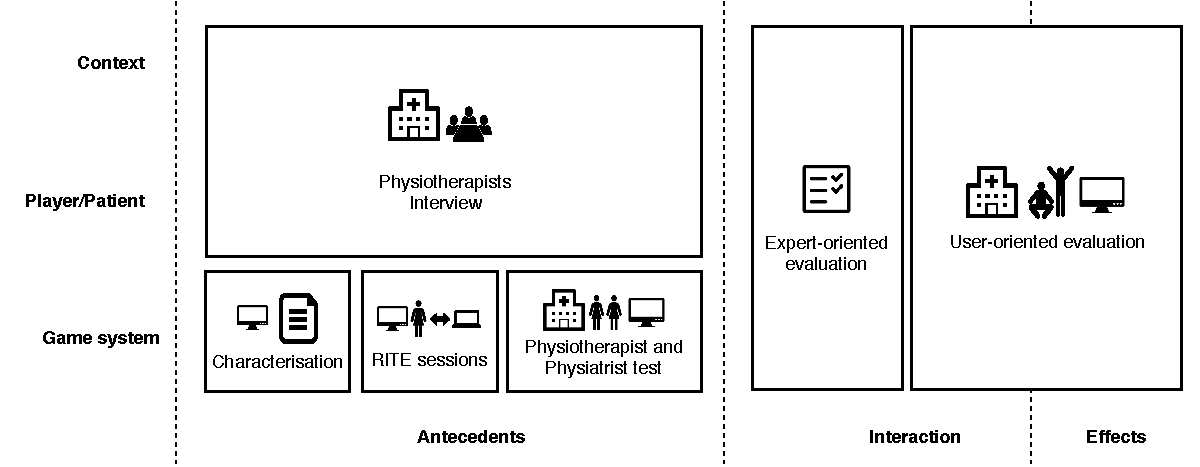
\includegraphics[width=\linewidth]{gfx/playtherapy/playtherapyEvaluation}} \quad
\caption{Overview of the evaluation of Playtherapy using the \ac{PX} model proposed in \autoref{ch:model}}
\label{fig:playtherapyEvaluation}
\end{figure}


The remaining of this chapter is organised as follows. First, we present the evaluation the antecedents of Playtherapy's mini \acp{PREG} regarding the context, player/patient and game system layers of \ac{PX}. Second, we present the evaluation of the interaction and effects of each mini \ac{PREG} throughout the three abstraction layers. Third, we present a discussion of the obtained results describing their implications and limitations. Also, we present recommendations for future work. Finally, we summarise and conclude the chapter.

\section{Antecedents}
We conducted three semi-structured interviews with three physiotherapists (2 female, 1 male) from the Evaristo Garc\'ia University Hospital. We obtained informed consents from the participants verbally. The interviews were audio recorded. The goal of the interviews is to collect information about the \emph{context} where they will use Playtherapy, their expectations regarding its use and the \emph{patients' profile}. Furthermore, the game system was characterised identifying Playtherapy's architecture and using the approach presented in \autoref{sec:characterising}. Additionally, two members of the development team, a physiotherapy student and a programmer, evaluated each mini-game using the \ac{RITE} method. A summary of the evaluation process is presented in \autoref{tab:antecedents_evaluations} and detailed in the following sections.

\begin{table}[bth]
\myfloatalign
\caption{Conducted evaluation sessions to evaluate antecedents of Playtherapy}
\resizebox{\linewidth}{!}{
\begin{tabular}{p{1.5cm}p{4.5cm}p{4.5cm}p{4cm}p{4.5cm}p{1.8cm}}
%----------------------
\toprule
\spacedlowsmallcaps{Layer}
& \spacedlowsmallcaps{Goal}
& \spacedlowsmallcaps{Aspects}
& \spacedlowsmallcaps{Methods}
& \spacedlowsmallcaps{Participants}
& \spacedlowsmallcaps{Sessions} \\\midrule
Context
& Identify the profile of physiotherapists from the hospital and the hospitals' regulations required to perform an evaluation
& Rehabilitation environment
& \multirow{2}{4.5cm}{Interview, Persona modelling}
& \multirow{2}{2.5cm}{3 physiotherapists}
& \multirow{2}{*}{2} \\\cline{1-3}
Player/ Patient
& Identify a general profile of patients from the hospital
& Player profile &  &  &  \\\midrule
\multirow{3}{1.5cm}{Game system}
& Characterise Playtherapy's mini-games
& Characteristics
& Characterisation \autoref{sec:characterising}
& 1 \ac{PX} evaluator
& - \\\cline{2-6}
& \multirow{2}{4.5cm}{Assess whether Playtherapy meets the requirements to be used by patients}
& \multirow{2}{4.5cm}{Configuration capability, Tutorial quality, Movement support}
& \ac{RITE}
& 1 physiotherapy student, 1 programmer
& 10 \\\cline{4-6}
&  &  & Question asking protocol
& 1 physiotherapist, 1 physiatrist
& 5\\ \midrule
\bottomrule
\end{tabular}}
\label{tab:antecedents_evaluations}
\end{table}

\subsection{Context}
As described in \autoref{sec:rel_among_dimension}, the context layer comprises the cultural parameters and the rehabilitation environment associated with the use of Playtherapy. To collect data about context, we use the following guiding questions for the conducted semi-structured interviews:

\begin{enumerate}
    \item What activities occur during physical therapy sessions?
    \item How can a \ac{PREG} be used as part of physical therapy?
    \item How do you expect to use \ac{PREG}?
    \item How do you think \acp{PREG} should assist patients?
    \item What kind of devices and software do you use on a regular basis?
\end{enumerate}

\subsubsection{Cultural parameters}
Regarding \emph{cultural parameters}, the physiotherapists have not used \acp{PREG} in the hospital; thus, we did not identify local game communities. Some of the physiotherapists have used commercial \acp{PREG} for their entertainment and outside the hospital. Only the academic community would represent an environment to share experiences and find relevant information. 

\subsubsection{Institution}
Regarding the \emph{rehabilitation environment}, the physiotherapists expressed that a typical rehabilitation therapy starts with an evaluation or diagnosis session, which will serve as input to establish rehabilitation goals and a treatment plan. A diagnosis session is performed according to the \ac{APTA} and the \ac{ICF} and may involve assessing aspects such as motion range, functional Independence, oxygen saturation, \ac{HR}, fine motor skill, balance, resistance and strength. During a rehabilitation treatment, physiotherapists perform re-evaluations periodically to assess patients progress and adapt treatment plan accordingly (e.g. by including new exercises or physical instruments). Patients' progress is tracked using forms established by the hospital. That confirms the relevance of the therapy tasks presented in \autoref{sub:def_rehab_therapy}; i.e., personalisation, supervision and assessment since they allow physiotherapists to determine whether a patient can use Playtherapy or not.

A therapy session takes one hour and comprises warm-up, cool-down and main therapeutic exercises, which are planned by a physiotherapist. In the first session, physiotherapists instruct patients to maintain a correct posture, avoid unsafe movements and take adequate precautions during exercises. Also, physiotherapists should explain and supervise each exercise execution specifying how to perform it correctly. At the end of each session, physiotherapists give feedback to patients and register important observations on a form. Moreover, auxiliary staff assist physiotherapists supervising and instructing patients. The decision to include a Playtherapy mini-game in a therapy session relies mainly on physiotherapists' criteria based on evaluation and re-evaluation results.

Playtherapy would be used in the Physical medicine and rehabilitation unit of the hospital. It has different facilities including a walk training area, a gym, a physical agents area, children area and adults area. Some of these places are usually crowded; thus, the location to use Playtherapy should be selected carefully. The unit is trying to provide two rooms to be used exclusively for playing Playtherapy.

Also, we identified internal regulations and constraints which are important to conduct an evaluation successfully. We need the approval of the head of the physical medicine and rehabilitation unit and the ethical committee of the hospital. A physiotherapist will be in charge of internal processes and logistics such as location, date, time, hospital participants and health instruments when needed. We should provide and coordinate the technical logistics. When an evaluation requires patients' participation, we should inform the physiotherapist at least four weeks in advance to arrange an appointment; otherwise, two weeks in advance would be enough. Finally, for long-term evaluations involving patients, we need the approval of the technical committee of the physical medicine and rehabilitation unit.

\subsubsection{Physiotherapists}
About \emph{physiotherapists profile and expectations}, they expressed that they feel confident using technologies since they are used to interact with smart-phones, computers and tablets. One of them has played exergames with Kinect One and Nintendo Wii. Another physiotherapist considered herself a casual player. The physiotherapists remarked that they are in charge of deciding what a patient can do in a therapy session since they are responsible for patients' safety. The physiotherapists expect Playtherapy to add variety and dynamism to the therapies they conduct, aid patients to reach the rehabilitation goals, motivate patients to perform the expected rehabilitation movements while reaching game goals, provide patients with information about goals, performance and progress. Moreover, they require Playtherapy to be an assisting tool that can be configurable to patients' needs and preferences (to assure patients' safety) and offer the possibility to work on particular joints and movements. They do not want Playtherapy to increase their workload. \autoref{fig:physio_personas} presents the two persona models that we built based on collected information.

\begin{figure}[bth]
\centering
 \subfloat[Physiotherapist with average IT mastery]{
   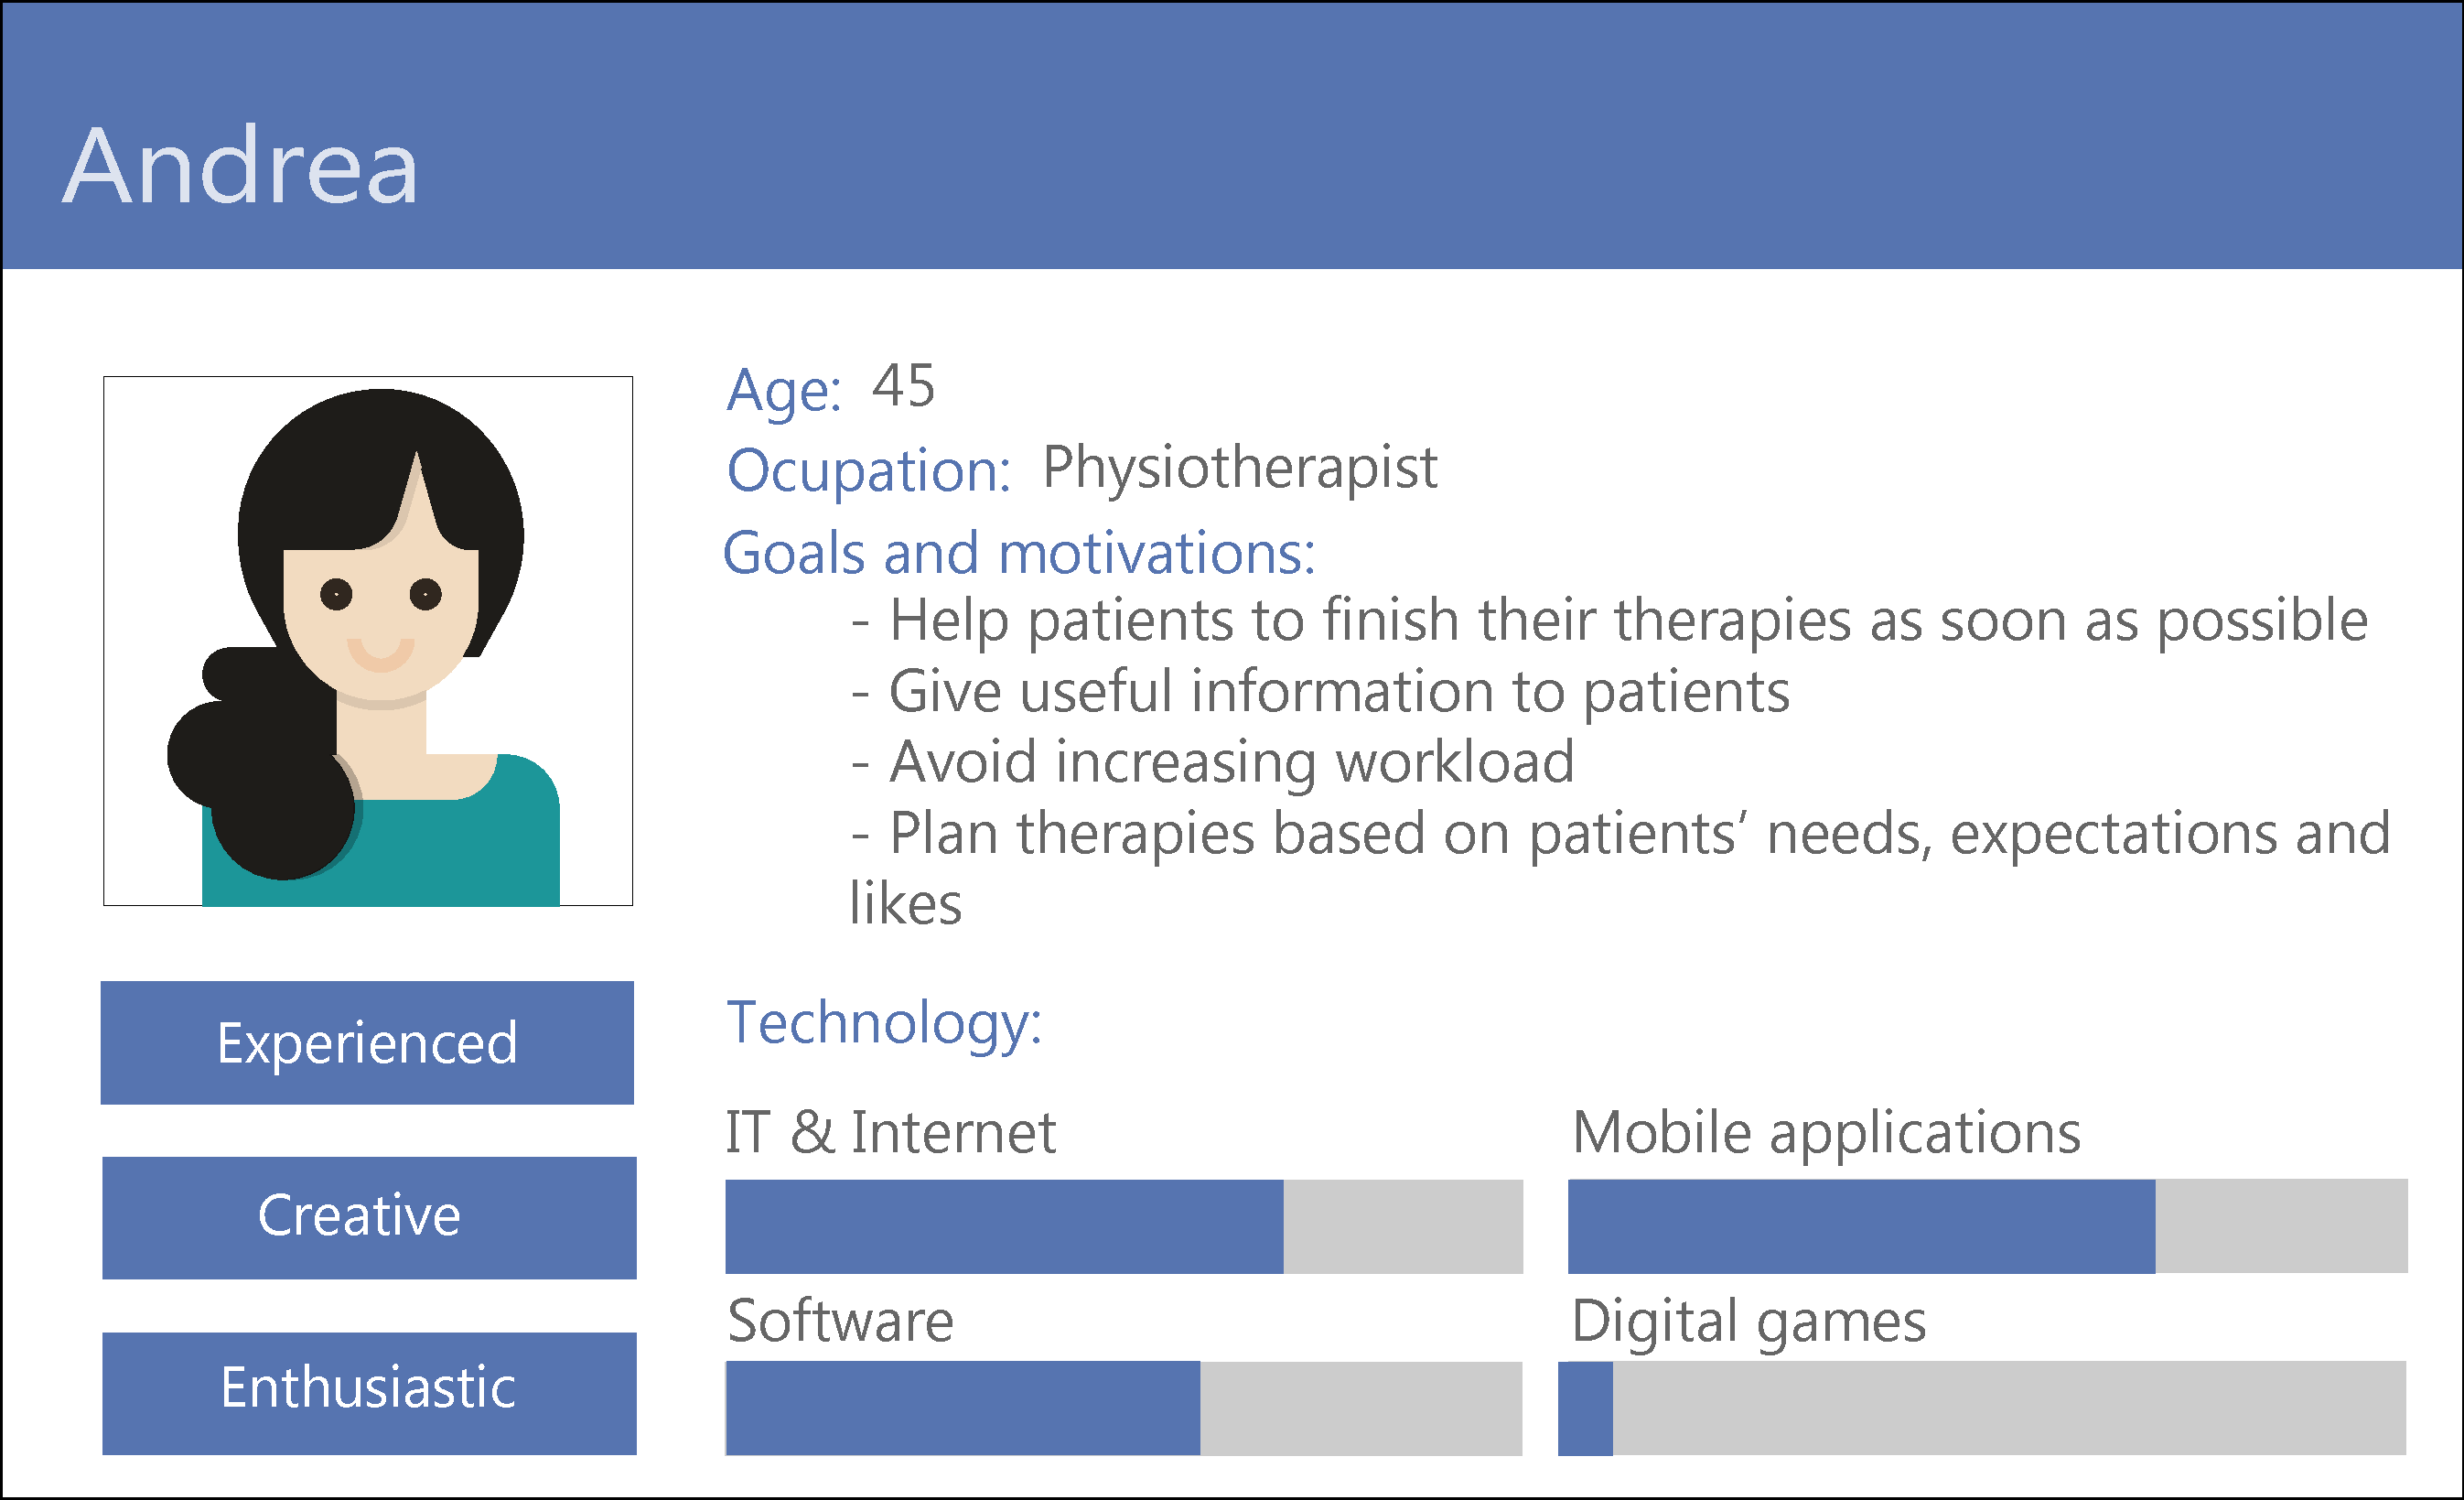
\includegraphics[width=0.48\linewidth, frame]{gfx/playtherapy/personaPhyAndrea}
   \label{fig:personaPhyAndrea}
 }
 \subfloat[Physiotherapist who sympathises with games]{
   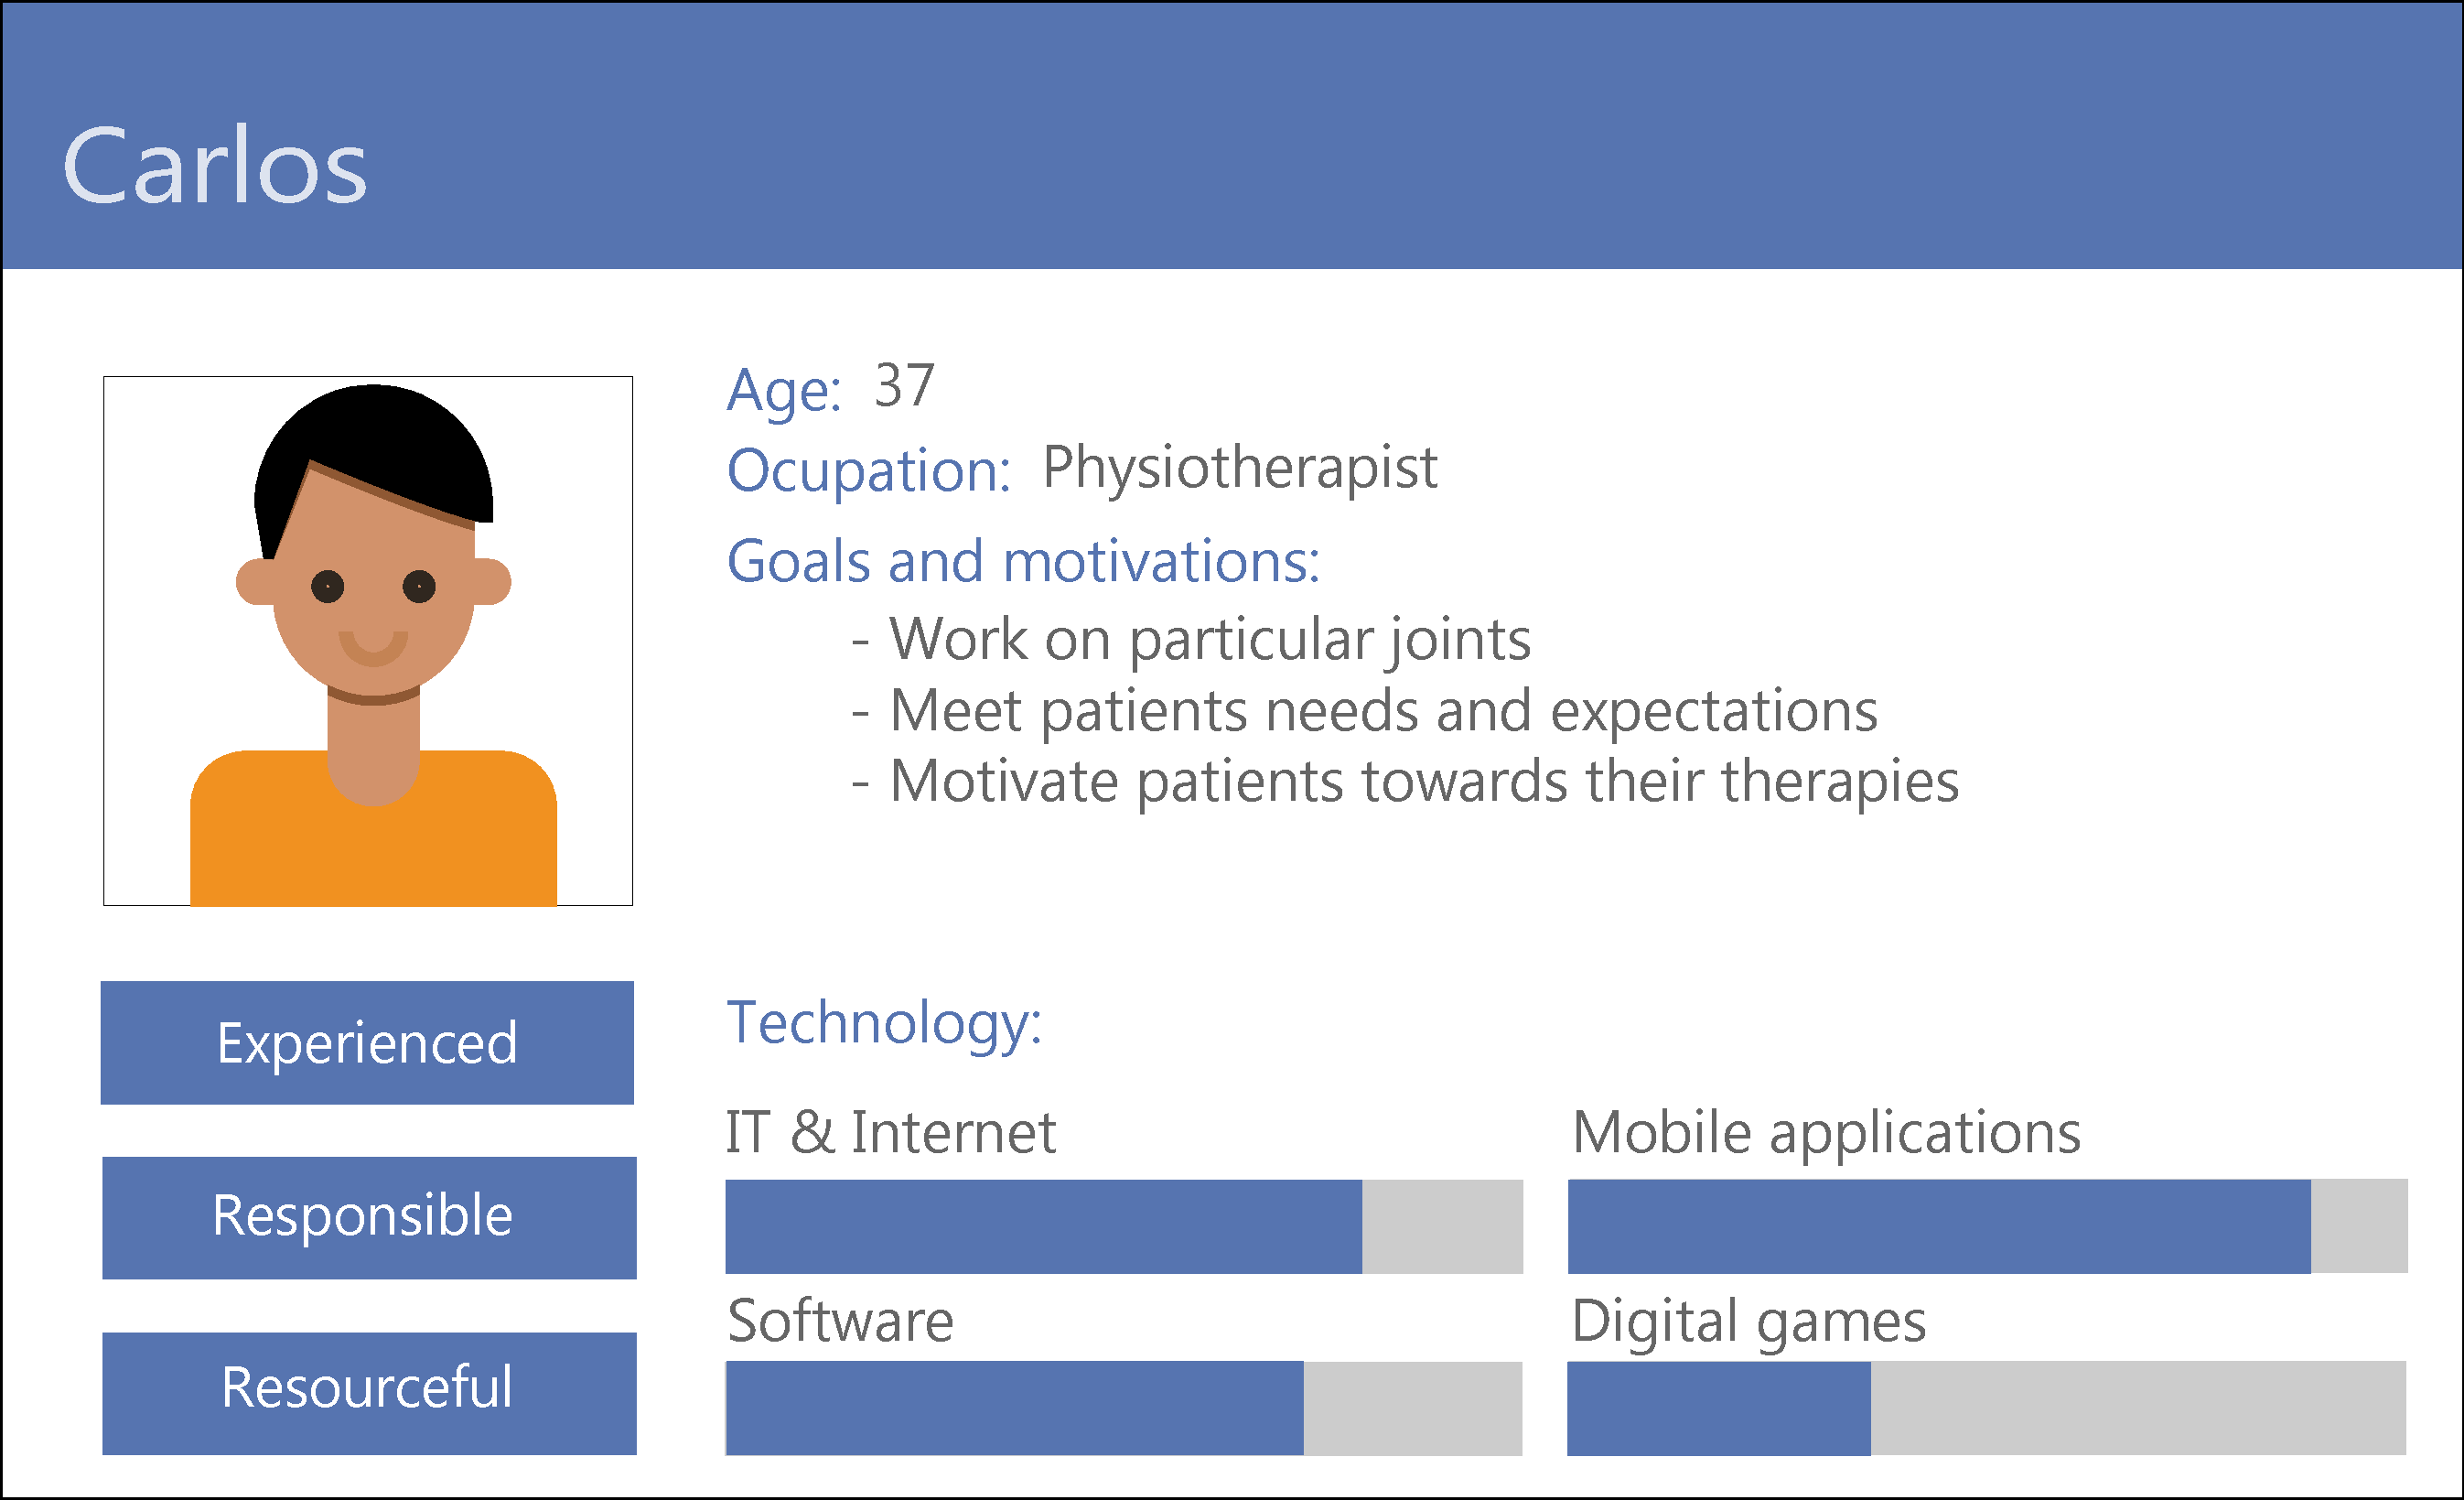
\includegraphics[width=0.48\linewidth, frame]{gfx/playtherapy/personaPhyCarlos}
   \label{fig:personaPhyCarlos}
}
\caption{Physiotherapists' persona models}
\label{fig:physio_personas}
\end{figure}

\subsection{Player/Patient}
Following the proposed model \autoref{sec:rel_among_dimension}, we identified characteristics, motivations and expectations of patients of the hospital to build Persona models (See \autoref{fig:patient_personas}). We use the following guiding questions to collect the data:

\begin{enumerate}
    \item What kind of patients do participate in physical therapy?
    \item How is patients' motivation towards physical therapy?
    \item What factors affect patients' motivation towards physical therapy?
\end{enumerate}

Specific information about \textit{game activity}, \textit{health status} and \textit{previous experiences} of players is collected before conducting any evaluation of \emph{Interaction} that involves patients (See \autoref{sec:eval_int_eff_participants}).

\subsubsection{Demographic characteristics}
The physiotherapists expressed that patients who require physical therapies have musculoskeletal, cardiopulmonary and neuromuscular impairments including lower and upper limbs fracture or traumas, cerebral palsy, joint dislocation and stroke. In the case of Playtherapy, it would be targeted at musculoskeletal patients since they require active exercises. Chronic patients are those who have a very limited range of motion of one or more joints.

Regarding age, the physical medicine and rehabilitation unit of the hospital treats children whose age range from 5 to 12 years. However, most patients are over the age of eleven. Also, young patients (13 - 17 years), young adult patients (18 - 35 years), adults (36 - 60 years) and elderly patients (older than 60 years) are treated.

Most children who are treated at the unit are attending primary school. Most young patients have finished primary school and attend secondary school, though, some of them quit before finishing it since they start working. Most young adults have finished secondary school or are finishing it. Some of them have completed a technical career. Most adult and elderly patients have finished at most primary school. Few of the adults have finished secondary school.

Most children who are treated at the unit are attending primary school. Most young patients have finished primary school and attend secondary school, though, some of them quit before finishing it since they start working. Most young adults have finished secondary school or are finishing it. Some of them have completed a technical career. Most adult and elderly patients have at most finished primary school. Few of the adults have finished secondary school.

The unit treats female and male children proportionally. Young and young adult patients are mainly male. Meanwhile, adult and elderly patients are mostly female. All patients belong to the lower or working classes; i.e., one, two and three Colombian social strata.

Regarding patients' disposition during therapy, the physiotherapists commented that children and young patients are willing to work during the therapy sessions and understand what they should do easily. Young adults and adults do not like reading and prefer visual aids. Finally, physiotherapists should monitor elderly patients closely since they have comprehension difficulties and get confused with the instructions easily.

\subsubsection{Motivations and expectations}

The physiotherapists remarked that patients' highest expectation is to finish a therapy as soon as possible. Other expectations include knowing the expected duration of their therapies and getting information about their impairment.

Regarding motivation towards a physical therapy, the physiotherapists highlighted that having an external reason to rehabilitate; e.g., to continue working or practising a sport, is a common source of motivation for patients. Also, patients get motivated when they feel that they are progressing in their rehabilitation goals; in that case, they start requesting more challenging activities and working independently at home to achieve more progress.

On the other side, the physiotherapists said that patients find physical exercises repetitive and monotone, which leads to a lack of motivation. Physiotherapists address that by including new activities, increasing exercises difficulty, including physical objects, among others. They highlighted that those activities rely on the creativity of the physiotherapist who is leading a treatment.

Additionally, patients have different sources of motivation depending on their age. Children are motivated by playful activities and visual aids: They want variety and find boring to focus on one activity; thus, physiotherapists should be very recursive. Meanwhile, young patients enjoy talking about trends and topics that they find interesting. They also like didactic material. Regarding young adults and adults, they prefer group activities over working individually such as sports or yoga classes.

\begin{figure}[tbh]
\centering
 \subfloat[Young patient]{
   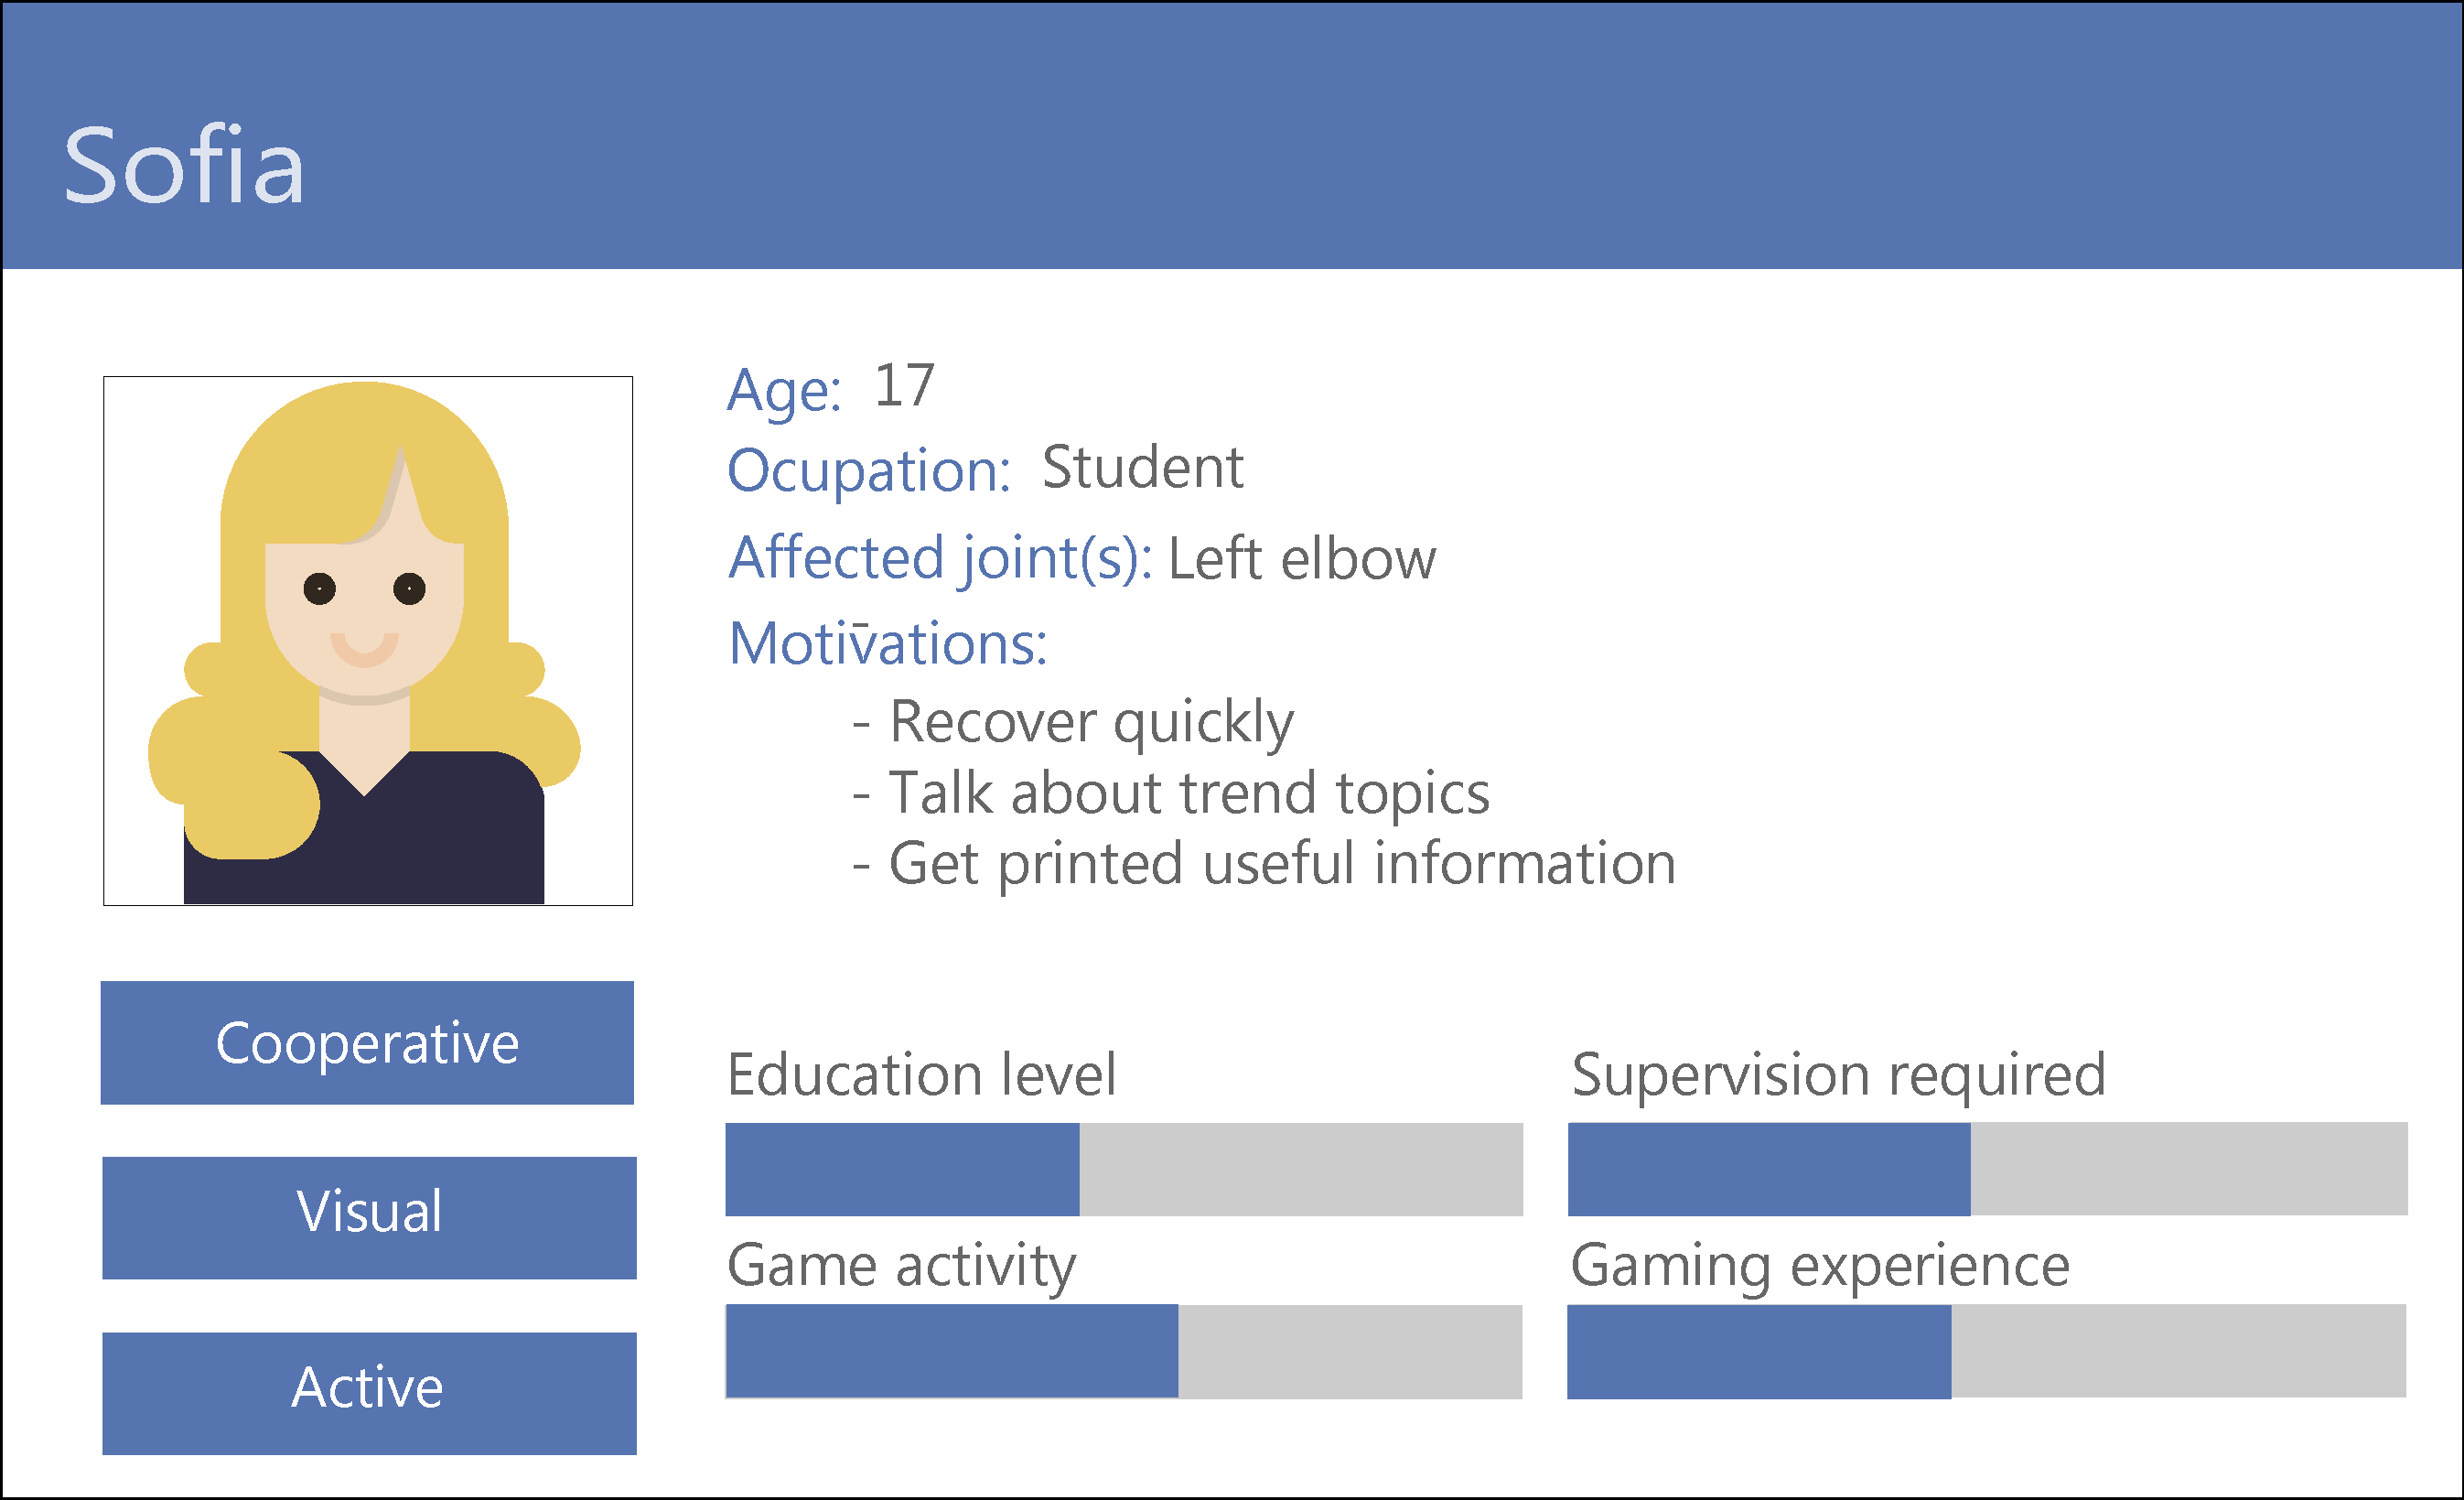
\includegraphics[width=0.48\linewidth, frame]{gfx/playtherapy/young_Persona}
   \label{fig:young_persona}
 }
 \subfloat[Young adult patient]{
   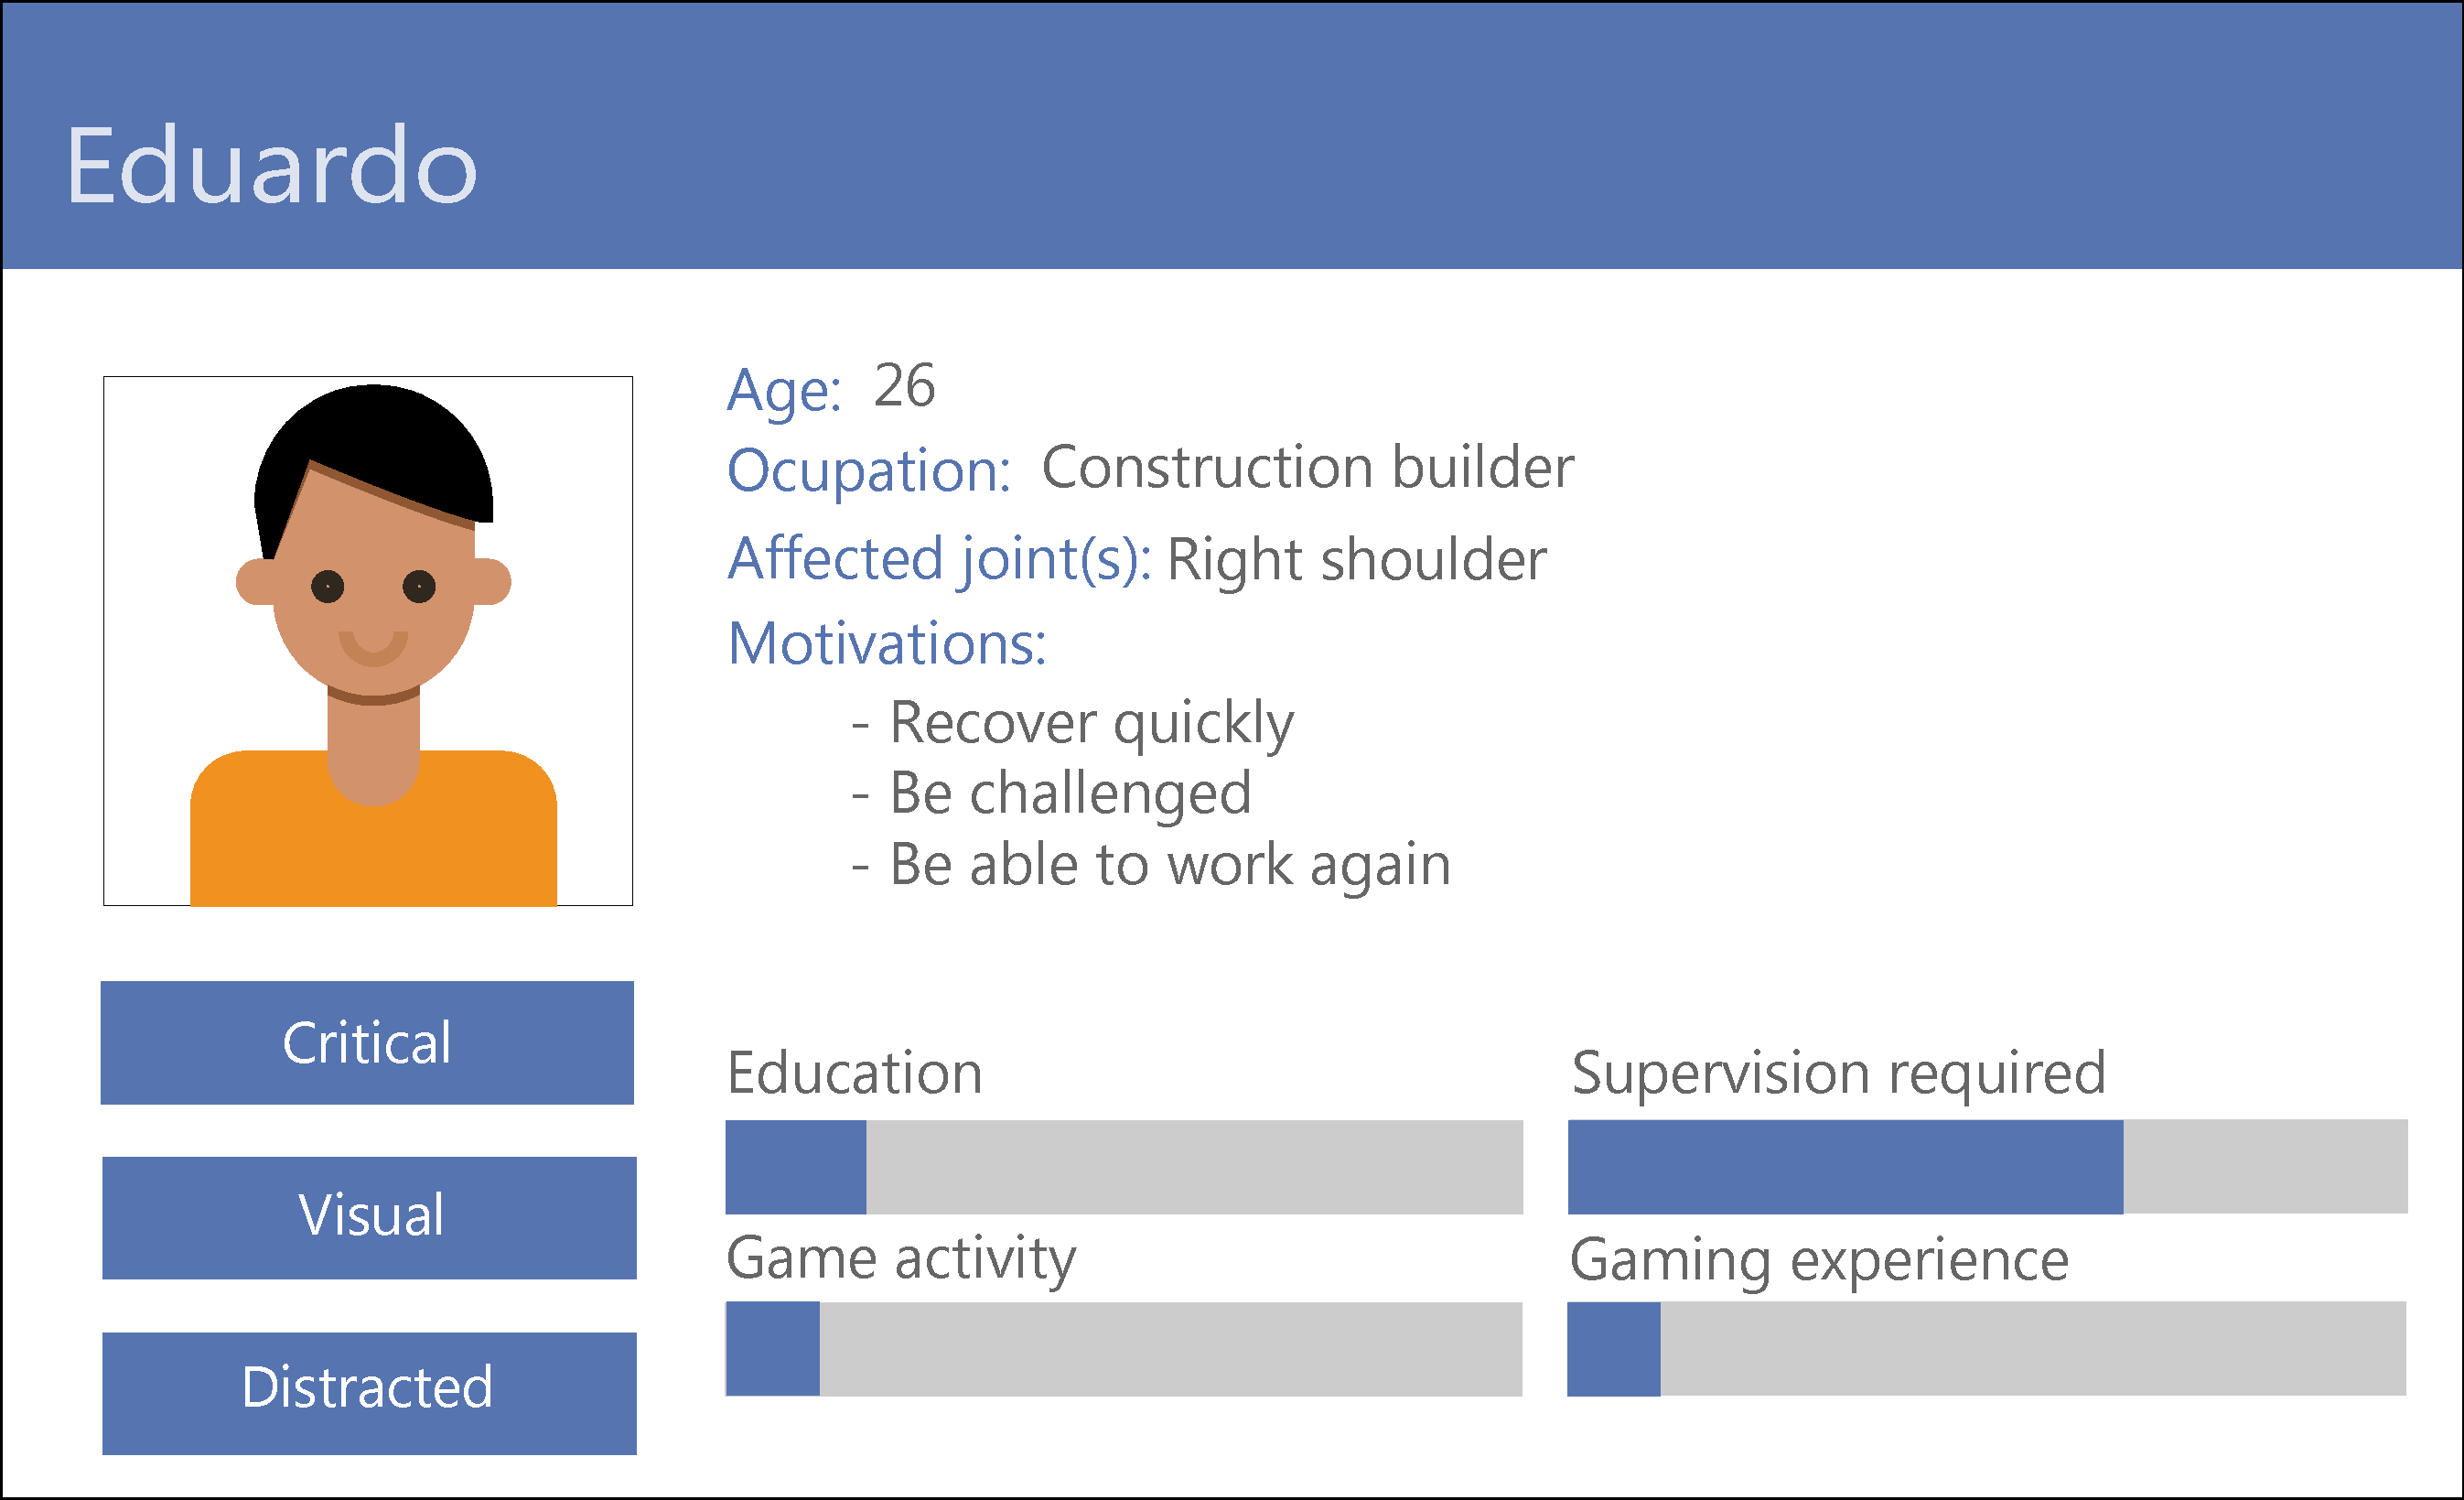
\includegraphics[width=0.48\linewidth, frame]{gfx/playtherapy/young_adult_Persona}
   \label{fig:young_adult_Persona}
}\\
\subfloat[Adult patient]{
   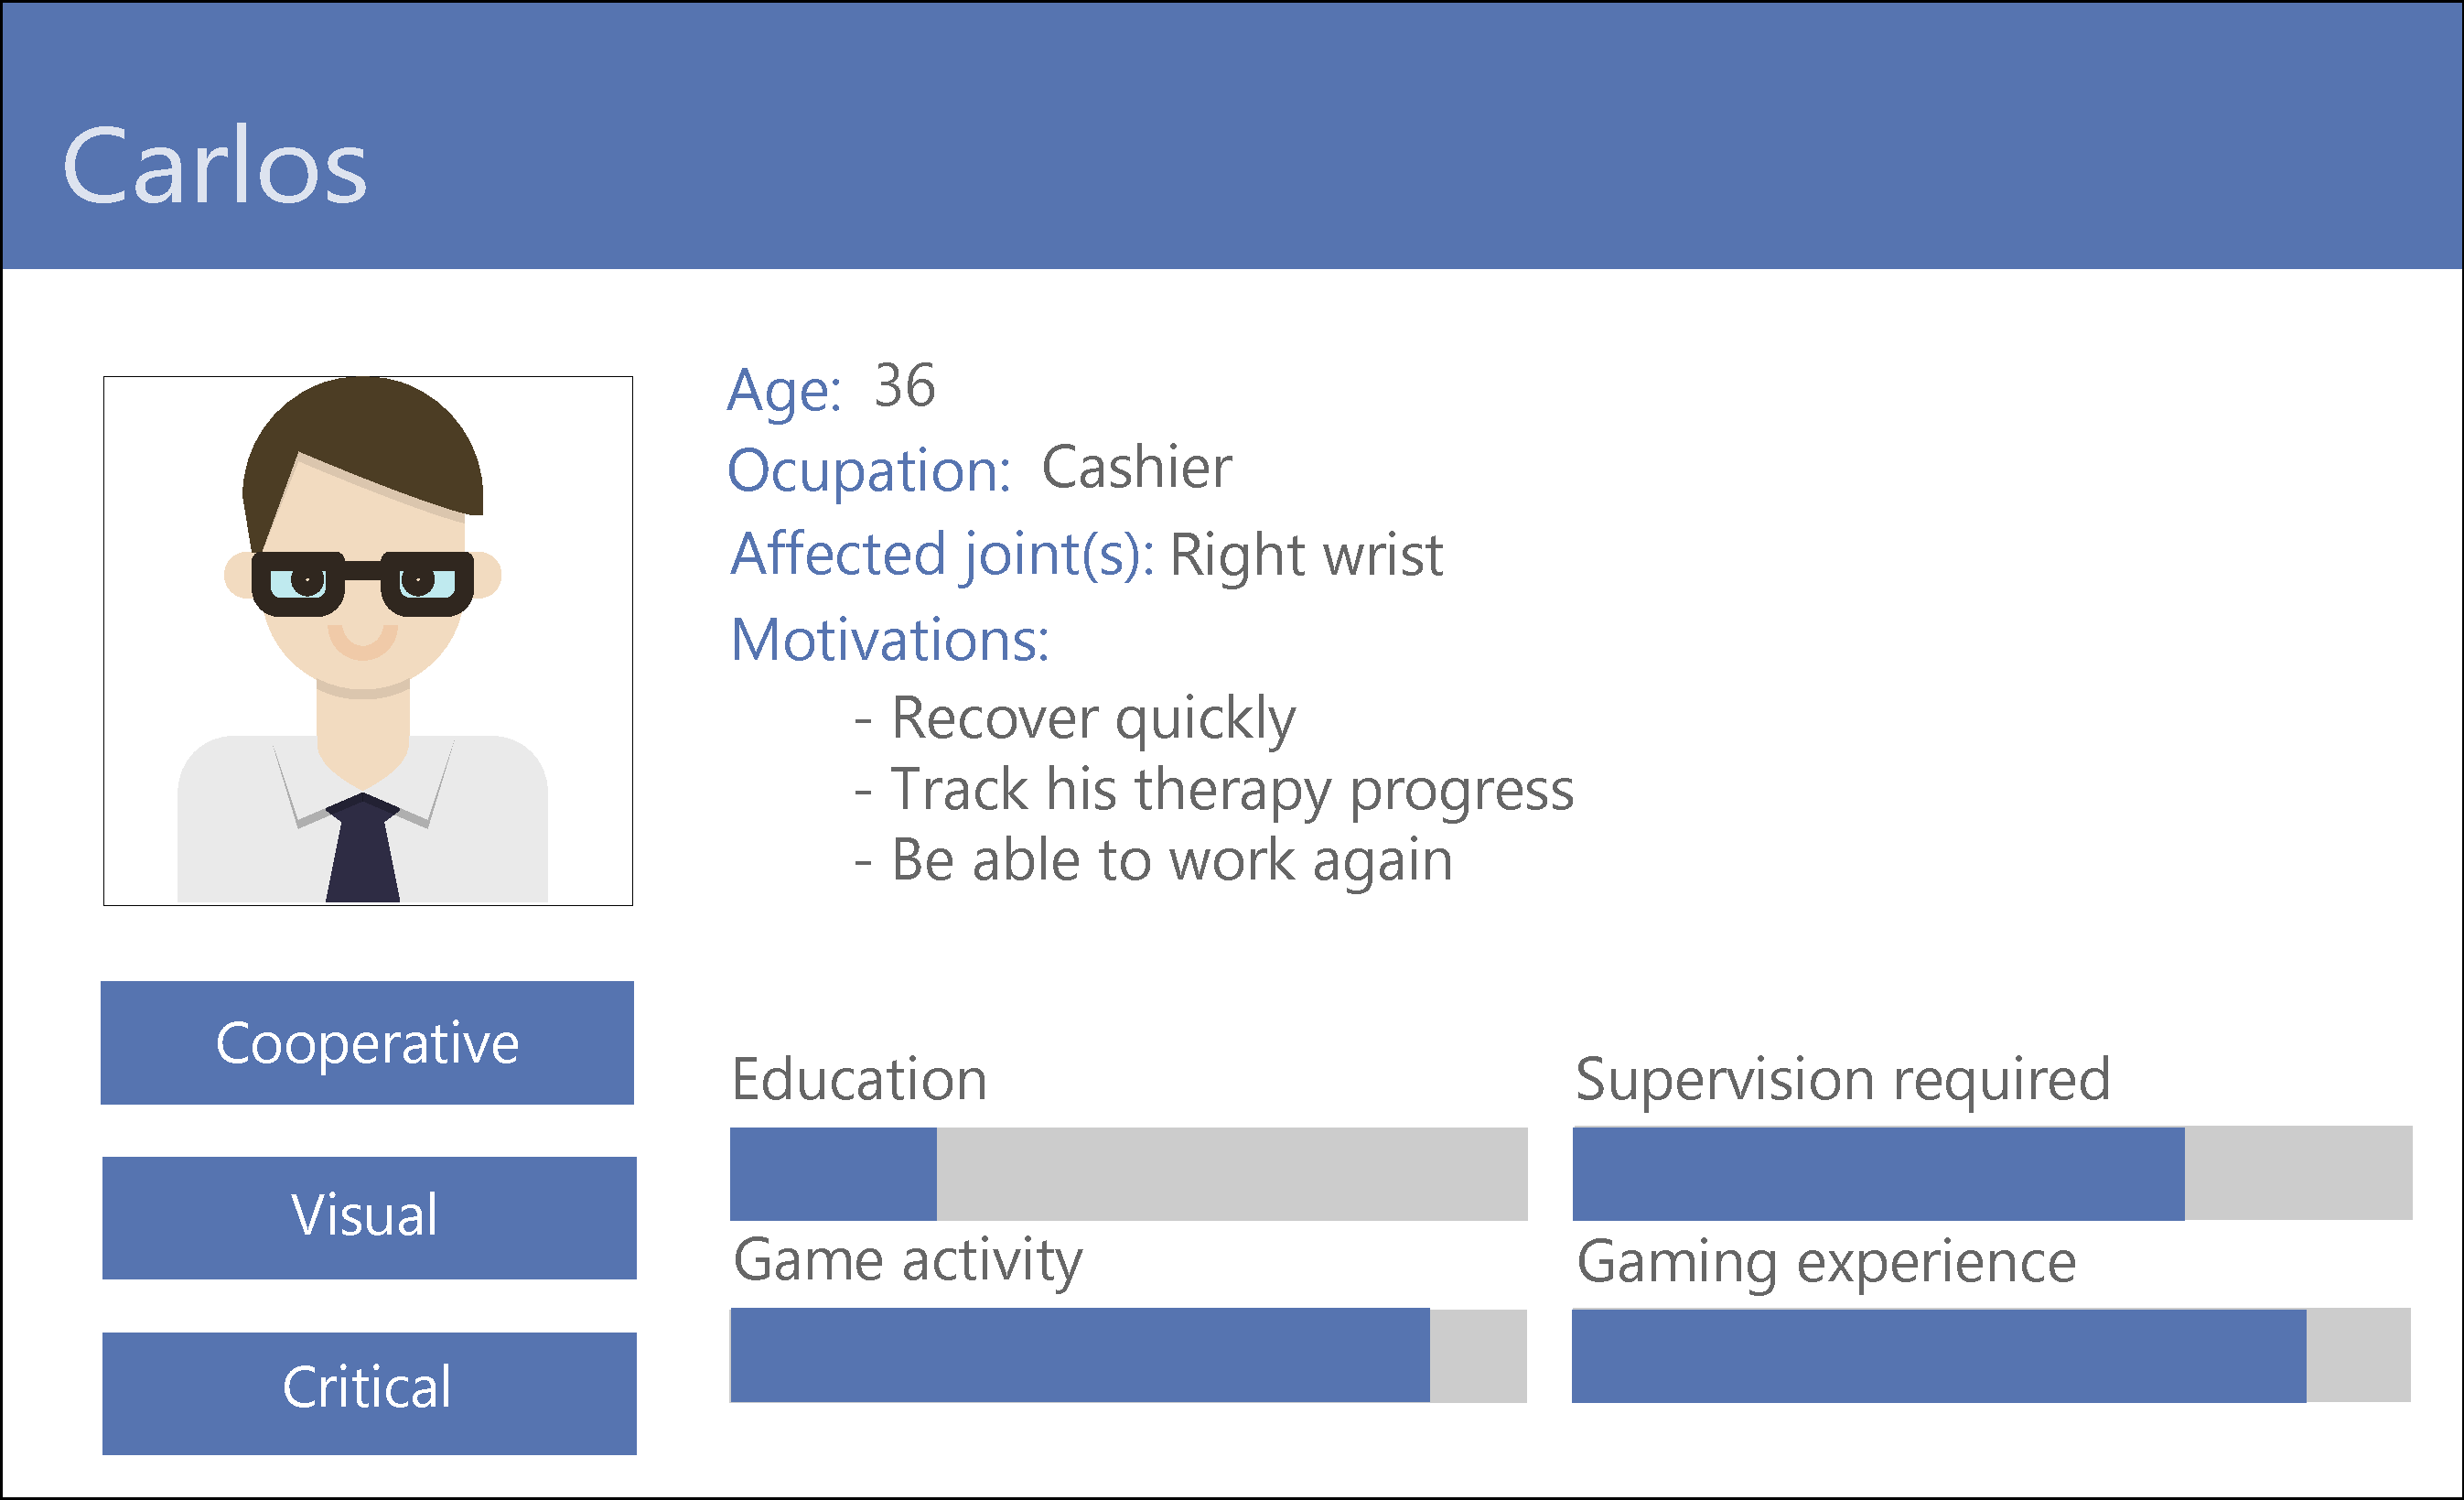
\includegraphics[width=0.48\linewidth, frame]{gfx/playtherapy/adult_Persona}
   \label{fig:adult_Persona}
}
\subfloat[Old patient]{
   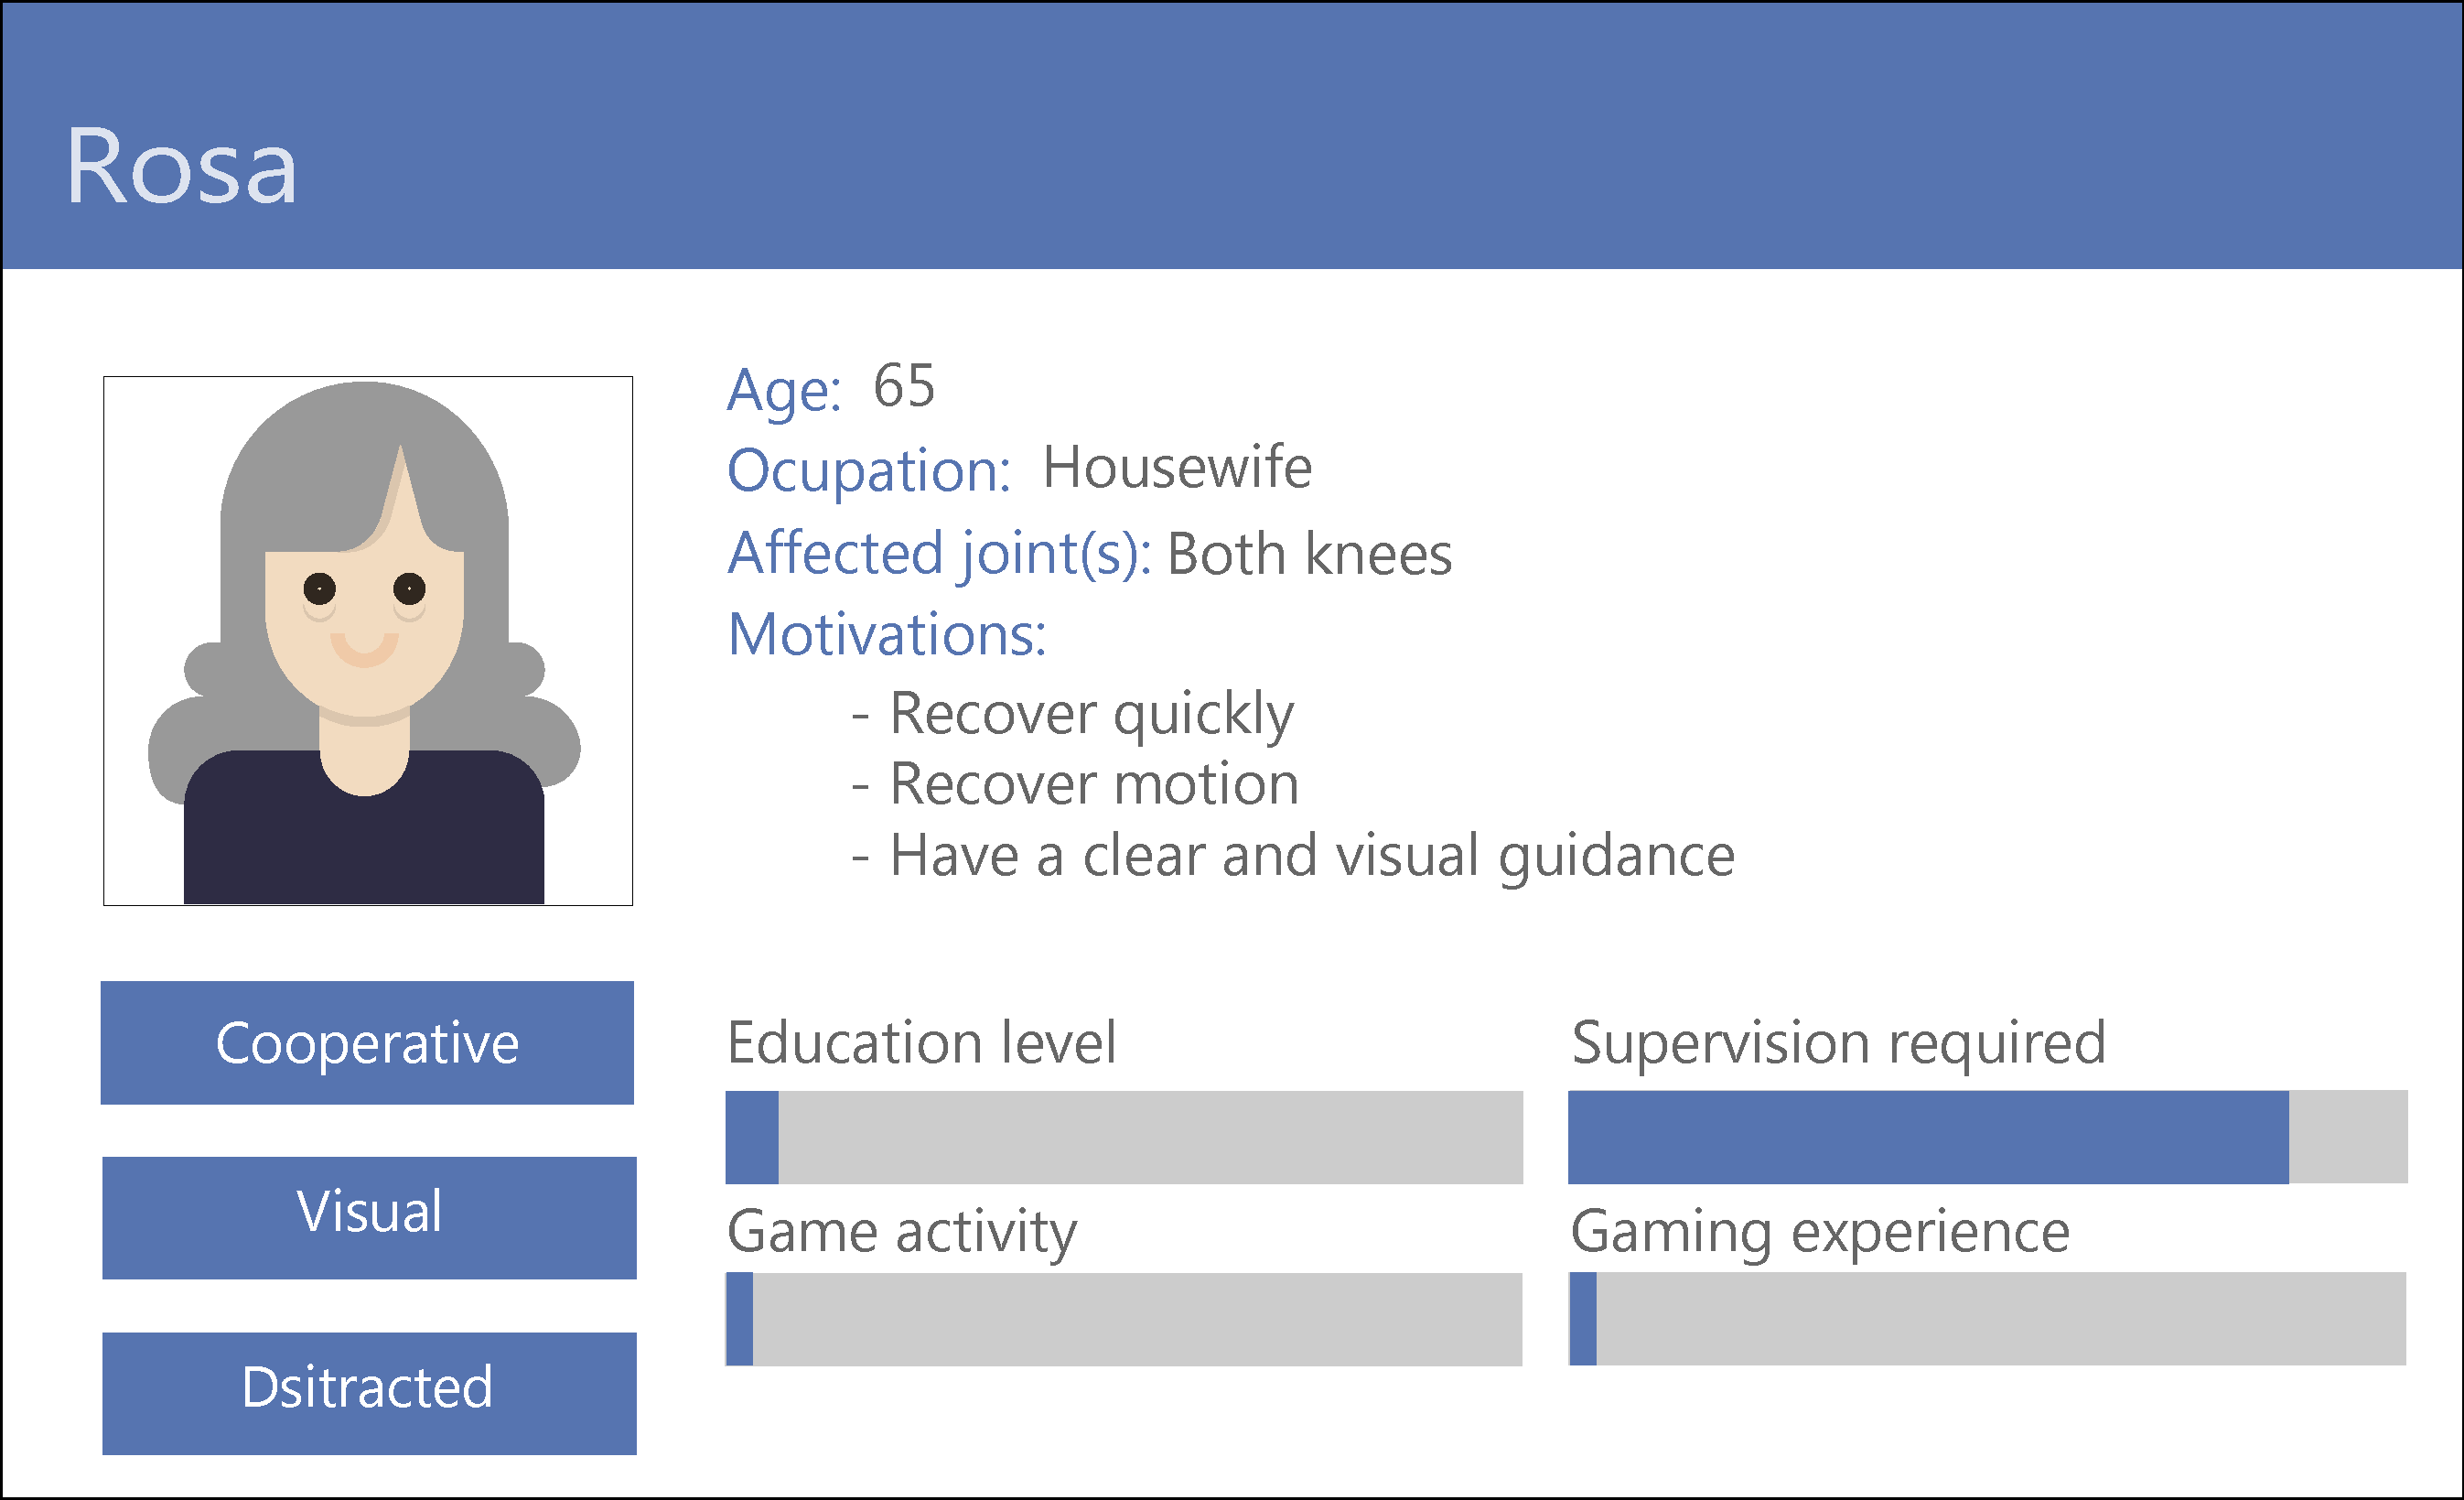
\includegraphics[width=0.48\linewidth, frame]{gfx/playtherapy/old_Persona}
   \label{fig:old_Persona}
}
\caption{Patients' persona models}
\label{fig:patient_personas}
\end{figure}

\subsection{Game system}

\subsubsection{General characteristics}
Playtherapy is a collection of mini \acp{PREG} whose purpose is to increase patients' motivation towards completing their physical rehabilitation therapies. Playtherapy is being developed by the Multimedia and Computer Vision research group from \textit{Universidad del Valle} in collaboration with the Physical Medicine and Rehabilitation Unit of the Evaristo Garc\'ia University Hospital from Cali Colombia. 

Playtherapy's mini \acp{PREG} are designed to assist patients to recover motion of particular joints, thereby being oriented to movements rather than impairments. It is a generic tool that may be used with patients having different impairments. As a consequence, two key elements of Playtherapy are the number of mini-games it contains and the coverage of joints it supports.

Playtherapy is being developed following an iterative and incremental methodology, which is appropriate for game development. The methodology is called Game-Scrum and consists in developing digital games using SCRUM agile practices along three stages: pre-production, production and post-production \autocite{godoy2010game}.

During \emph{pre-production} developers define an initial and general idea for the game, it comprises, among other aspects, its characteristics, rules, controls, art and sound. Developers perform activities such as brainstorming, prototype development, game sessions and technologies exploration are performed. The outcome of this stage is a \ac{GDD}. Then, in \emph{production} stage, developers define the game's \textit{product backlog} using the \ac{GDD} of the previous stage as input. This phase progresses following the roles, artefacts and meetings of SCRUM \autocite{keith_agile_2010}. Finally, \emph{post-production} includes evaluating the game being developed and the creation of a \textit{postmortem} to collect learned lessons that can be used in future projects.

Each mini \ac{PREG}, including its thematic, main objectives, rules and mechanics were designed during weekly brainstorming sessions involving the participation of a physical therapy undergraduate student. Additionally, regular meetings with a group of physiotherapists from a local hospital were arranged, where continuous feedback was received to develop, validate and improve every implemented feature; so that the mini \acp{PREG} could meet both physiotherapists' and patients' needs.

Playtherapy is developed in an academic environment. The defined sprint length for the project is two weeks. As expected, a sprint planning, a sprint review and a retrospective meeting are performed every sprint. The development team is composed as follows:
\begin{itemize}
    \item \emph{System engineering undergraduate students}: they are responsible for the video game implementation; i.e., they develop every user story related to the project. Also, they are responsible for performing functional testing and adapt Playtherapy according to the results obtained after user acceptance tests and \ac{PX} evaluations performed with physiotherapists and patients. In the context of SCRUM methodology, those students play the role of development team members.
    \item \emph{Physiotherapy undergraduate student}: she is responsible for guiding the previous team in aspects related to the physical rehabilitation field. Further, she approves acceptance tests and participates in the validation of the employed technologies and mini \acp{PREG}. According to SCRUM, that student plays the role of a development team member.
    \item \emph{Systems engineering master student}: he is responsible for leading the development process, coordinating every meeting and practice proposed by the SCRUM methodology. He plays the role of a SCRUM master role.
    \item \emph{Physiotherapist}: a physiotherapist participates in every sprint review meeting to validate all implemented features and guarantee that the mini \ac{PREG} meets the patients' needs. His/her role is \textit{product owner} according to SCRUM methodology.
\end{itemize}

All team members participate in generating ideas to design and implement each mini \ac{PREG}. The goal of having an interdisciplinary team is to explore different possibilities and validate their viability regarding physical rehabilitation needs and technology capabilities.

\subsubsection{Characteristics of the mini \acp{PREG}}
Playtherapy covers a set of rehabilitation movements and exercises using mini \acp{PREG} that support specific joint movements. Each mini \ac{PREG} is designed to be personalised by physiotherapists to adapt to patients' needs and offer a compelling and natural experience. A mini \ac{PREG} comprises a set of components, which were created to assist physiotherapists work and enhance patients' experience when interacting with a mini-game. These components are illustrated in \autoref{fig:mg_arch}.

The \emph{GUI} component is composed of the screens that each mini \ac{PREG} has. Each screen was created following a standardised design pattern and usability guidelines related to colour and elements distribution. There are three main screens. First, the \emph{parameters screen} which allows physiotherapists to set up a mini \ac{PREG} before it starts to adapt the game session to patients' particular needs (See \autoref{fig:parameters_screen}). A mini \ac{PREG} is configurable through a set of parameters, such as movement angle thresholds, choosing between repetition based or session time-based session and enabling or disabling joints and exercises. Every parameter configuration was agreed on with the physiotherapists who supported the development process. Second, the \emph{tutorial screen} explains the game objectives, rules and mechanics (See \autoref{fig:tutorial_screen}). Additionally, the tutorial includes visual representations of the movements that a player/patient has to perform, which allows therapists and patients to understand how to play and interact with the game. Finally, the \emph{results screen} shows the performance obtained by a player/patient along with visual feedback after a game session (See \autoref{fig:results_screen}). The visual feedback is always positive since Playtherapy is a game intended to motivate and distract players/patients from their environment. Therefore, players/patients always receive a reward disregarding how well they perform.
    
The \emph{world} component comprises the elements related to the mini \ac{PREG} environment. These elements are mainly 3D models and materials that make up the background objects and interaction elements of the mini \ac{PREG} (See \autoref{fig:world_screen}). This world comprises the elements. First, the \emph{game scenario} includes all the background elements that constitute the world of the game, such as terrains, background nature and buildings, skyboxes, and any other non-interactive game objects. Second, the \emph{interaction elements} comprise specific objects that players interact with by performing different movements and exercises associated with the mini \ac{PREG}. Third, \emph{feedback effects} are triggered to help players/patients be conscious of the outcomes of their actions. Fourth, the \emph{final animation} indicates players/patients that a mini-game session has ended. The goal of this component is to provide a smooth and compelling transition from the game end and the Results Screen. This transition was denominated the Final Animation and consists in a sequence of game objects behaviours that dynamically and graphically illustrate the end of a game session.

The elements of the \emph{logic} component are mainly scripts that define the different rules, mechanics and behaviours of the mini \acp{PREG}. Logic is structured as follows, a \emph{game manager} controls mini \ac{PREG}'s flow and state. It determines and controls when the game starts, pauses and ends. It also keeps track of the current score of a player, updating it according to each player movement. It controls the mini \ac{PREG} behaviour according to configured parameters signalling corresponding events and actions. A \emph{movement control} component communicates with tracking devices' APIs to get the required data, such as joint position and rotation. Then, it performs corresponding calculations to determine if a player has performed a certain movement or exercise. A \emph{persistence} component stores patients' performance based on the obtained score and range of motion progression. This information is used by a web application, that belongs to Playtherapy, to generate reports.

\begin{figure}[h]
\centering
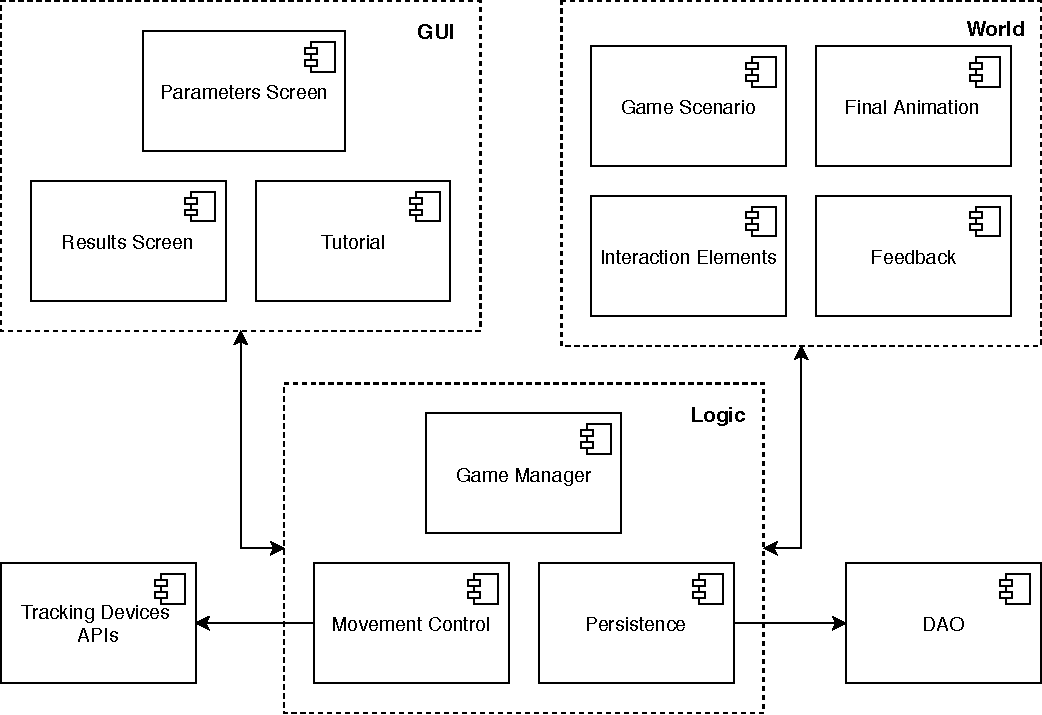
\includegraphics[width=.9\linewidth]{gfx/playtherapy/minigame_architecture}
\caption{Playtherapy's mini \acp{PREG} architecture}
\label{fig:mg_arch}
\end{figure}

\begin{figure}[bth]
\centering
\subfloat[\textit{Piano}'s parameters screen]{
   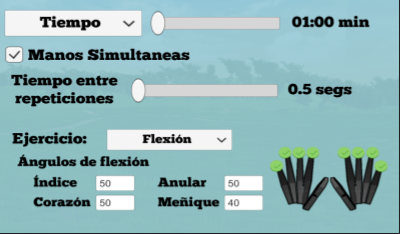
\includegraphics[width=0.4\linewidth, frame]{gfx/playtherapy/parameters_screen}
   \label{fig:parameters_screen}
}
\subfloat[\textit{Rieles}' tutorial screen]{
   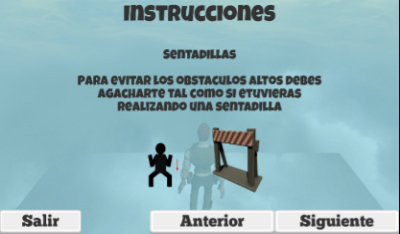
\includegraphics[width=0.4\linewidth, frame]{gfx/playtherapy/tutorial_screen}
   \label{fig:tutorial_screen}
}\\
\subfloat[\textit{Tiro Libre}'s results screen]{
   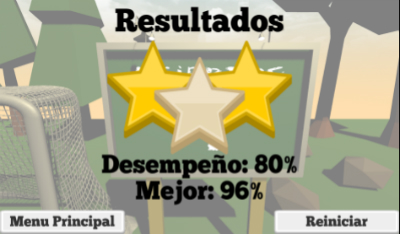
\includegraphics[width=0.4\linewidth, frame]{gfx/playtherapy/results_screen}
   \label{fig:results_screen}
 }
 \subfloat[\textit{Tiro Libre}'s game world screen]{
   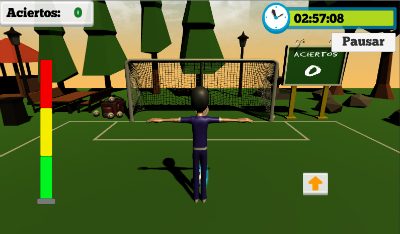
\includegraphics[width=0.4\linewidth, frame]{gfx/playtherapy/world_screen}
   \label{fig:world_screen}
}
\caption{Playtherapy's mini \acp{PREG} main screens}
\label{fig:platherapy_screens}
\end{figure}

Playtherapy is composed of fourteen mini-games which are briefly described below. Moreover, a characterisation of one the mini \acp{PREG} is presented in \autoref{tab:beisbol_char}, it uses the approach presented in \autoref{sec:characterising}. The characterisation for all mini \acp{PREG} is available online \footnote{Playtherapy's mini \acp{PREG} characterisation: \url{https://goo.gl/uaxqWa}}.

\begin{enumerate}
    \item \emph{Tiro Libre}: players perform kick movements to strike a ball against some targets placed in a goal. It should support right/left hip flexion and extension and lateral shifts.
    \item \emph{Rieles}: players jog to go forward and squat and jump to avoid obstacles while collecting coins. It should support jumps, squats, jogging and lateral shifts.
    \item \emph{El Gran Viaje}: players control a plane moving their body to collect gems and avoid obstacles. It should support right/left hip abduction, lateral and frontal trunk inclination and squats.
    \item \emph{F\'utbol Libre}: players have to maintain a ball in the air using their legs. It should support right/left hip flexion and extension.
    \emph{B\'eisbol}: players have to grab balls being thrown at them using their arms. It should support right/left shoulder abduction or extension, elbow flexion and extension.
    \item \emph{Defensa M\'agica}: players use their arms to perform magic tricks and defend the city. It should support right/left shoulder and elbow flexion and extension.
    \item \emph{Figuras M\'agicas}: players have to draw figures using their hands to eliminate approaching enemies. It should assist in hand-eye coordination.
    \item \emph{Piano}: players have to perform finger movements to play a piano keyboard. It should support fingers flexion, extension and oppositions.
    \item \emph{Topos}: players perform grabbing movements (fist) to catch moles or directly touch them by moving their hands. It should support hand touch and grab.
    \item \emph{Vecinos Invasores}: players have to defend farm animals from being abducted by destroying alien ships using their hands. It should support hand touch and fingers oppositions.
    \item \emph{Viajando en el Espacio}: players control a spaceship using their hands to collect stars and overcome obstacles. It should support ulnar and radial deviation, wrist flexion and extension and hand grab.
    \item \emph{Dulce Hogar}: players control a cat using their hands to collect stars and avoid enemies. It should support ulnar and radial deviation, wrist flexion and extension.
    \item \emph{Cavano}: players control a bowl using their hands to gather falling objects and drop them into a jar. It should support pronation and supination.
    \item \emph{Guerra Medieval}: players have to defeat enemies using hand movements. It should support ulnar and radial deviation, wrist flexion and extension and hand grab.
\end{enumerate}

Playtherapy uses two \textit{input interaction devices}; the mini \acp{PREG} that involve wrist and fingers movements use the Leap Motion \autocite{leap:2017}. The other mini \acp{PREG} use Kinect 2\autocite{kinect:2013}.

\begin{table}[bth]
\myfloatalign
\resizebox{.9\linewidth}{!}{
\begin{tabular}{p{5cm}p{10cm}}
%----------------------
\toprule
\spacedlowsmallcaps{Property}
&\spacedlowsmallcaps{Value}\\\midrule
Rehabilitation type & Tight-focused \\\midrule
Assisted Tasks & Configuration, personalisation and motivation \\\midrule
Degree of autonomy & Second degree \\\midrule
Configuration and assessment & Close-loop (Online motion range measurement)\\\midrule
Input interaction device & Camera tracking: Kinect 2\\\midrule
Output interaction device & Traditional: TV screen, speakers\\\midrule
Thematic content & Imaginary\\\midrule
Type of intervention & Individual \\\midrule
Location & Physical medicine and rehabilitation unit of Evaristo Garc\'ia University Hospital\\\midrule
Movements & Right/left shoulder abduction and/or extension, elbow flexion and extension\\\midrule
Configuration parameters & Game mode, left/right shoulder selection, minimum angle and maximum angle per movement, radius (reformulated as Movement action radius), ball speed\\\midrule
Rehabilitation goal(s) & Patient increases shoulder abduction or extension range of motion\\\midrule
Health instruments & Goniometer\\\midrule
\bottomrule
\end{tabular}}
\caption{Characterisation of \textit{B\'eisbol} mini \ac{PREG}}
\label{tab:beisbol_char}
\end{table}

Furthermore, Playtherapy has an accompanying web application composed of three main modules. The first module is concerned with patients and physiotherapists demographic data. The second module allows physiotherapists managing patients \ac{FIM}. Finally, the third module allows visualising mini-game sessions data; e.g., registered observations, progress over time and performance measurements, like the maximum range degree achieved per session. By the time this master project took place, this application was still under development and was not connected to Playtherapy; thus, it was not evaluated.

\subsubsection{Rehabilitation support}
As described in \autoref{sec:characterising} the rehabilitation support aspect comprises assessing movement support and configuration and personalisation capability. The goal of evaluating rehabilitation support is to assure that the evaluated \ac{PREG} can be used with patients safety. Before Playtherapy's mini \acp{PREG} that use Kinect were developed a feasibility study was conducted to identify the movements that were detected satisfactorily according to a group of physiotherapists. This study can be found in \autocite{Prado2018}. Similarly, a second study was conducted to identify acceptable hands movements detected by the Leap Motion \autocite{Lopez2017}.


We performed an \emph{internal evaluation} with two members of the development team, a physiotherapy student and a programmer, who conducted ten sessions of \ac{RITE} testing. The physiotherapy student tested all Playtherapy's mini \acp{PREG}. To assess \textit{configuration capability}, she tested each configuration parameter to assess whether it behaved as expected and was easy to understand. Moreover, she tested whether the expected \textit{movements were correctly mapped} and detected by each mini \ac{PREG}. Additionally, she evaluated the \textit{quality of the tutorials} assessing the content and the coverage of the associated movements regarding the game mechanics. When she identified an error or an enhancement, the programmer fixed it and the student test it again until it was correct.

The results of the \ac{RITE} evaluation were mainly improvements related to the phrasing of configuration parameters and tutorial instructions. The student assessed their clarity from the physiotherapists' and patients' point of view. Similarly, she suggested to include graphics or animations to make the instructions and movements clearer. She configured the games considering different (ad-hoc) scenarios, exploring different game modes, including and excluding movements and modifying their difficulty. While testing each scenario, she also assessed the visibility of game objects and relevance of the visual and auditory feedback related to the game goals, leading to the inclusion of visual animations and sounds (e.g., to indicate the corresponding joint to execute a certain movement).

After the internal evaluation, we conducted five evaluation sessions of one hour using the question asking protocol and involving one physiotherapist and on physiatrist of the hospital. The purpose of this evaluation stage was to validate the results of the evaluation conducted with the development team. Eight mini \acp{PREG} were tested in this evaluation; i.e., \textit{Béisbol, Defensa M\'agica, Tiro Libre, Guerra Medieval, F\'utbol Libre, Figuras Mágicas, Gran Viaje} and \textit{Vecinos Invasores}. The last eight of these mini \acp{PREG} had been tested by the physiotherapist; thus, fewer issues were identified for those.

The participants were asked to configure at least two game sessions for each mini \ac{PREG}. After configuring one game session, they played it to identify errors or improvements. The first configuration was suggested by the evaluator, and the others were proposed by the participants. During the whole process, they could express their thoughts and impressions loudly . The evaluator could ask questions when needed. We took notes of the findings during the evaluation.

Initially, \textit{Béisbol} mini \ac{PREG} had a name in English (Baseball); however, the participants suggested to use the same name in Spanish due to the low level of patients' literacy. They expressed that understanding the game name was important to understand the game. Also, they remarked that game should indicate the patients where they should position the avatar before starting the game; they suggested to include a position mark and ask patients to move towards it. Moreover, they requested to rename one of the configuration parameters from \textit{Ratio} to \textit{Action ratio} (in Spanish) for understanding purposes. This parameter indicates the distance between the thrown ball and the patients' hands, depending on its value patients should stretch their arms or perform elbow flexion and extension movements. They suggested some rephrasing for the tutorial instructions. Regarding, movement mapping correctness, all movements were mapped correctly. However, they detected that a reduced shoulder abduction could be detected as shoulder extension. Finally, they suggested to include a visual mark indicating the position where patients should catch the balls to foster correct movement executions.

Similarly, the participants suggested to rename \textit{Defensa M\'agica} since its original name was in English (Fight). Also, the game displayed some visual objects to determine whether the patient should perform elbow movements. However, this was not explained in the tutorial. Thus, they requested to include that information.

About \textit{Tiro Libre}' parameters screen, the participants requested to use the term coronal plane instead of frontal plane for one of the parameters. Also, they suggested to group the \textit{Lateral shifts} and \textit{Frequency} parameters visually since they are related. Additionally, they noticed that a bar that represented the final height of a kicked ball was placed horizontally and suggested position it vertically. In the tutorial, they suggested changing the figures to differentiate lateral from frontal movements. Also, the dynamic help offered by the game was not explained in the tutorial.

Regarding \textit{Guerra Medieval}, the participants suggested to visually separate two excluding parameters. Also, the screen allowed to include pronation and supination movements, however, the game mechanics do no use them. Thus, they requested to remove them. Although the players control a virtual cannon in the game, they suggested to include virtual hands to help players be conscious of the movements they are performing. Also, they identified some typos in the tutorial and suggested to include more graphical aids and reduce the amount of text.

They detected that the performance measure presented by \textit{F\'utbol Libre} at the of a game session was calculated incorrectly. About the tutorial, they noticed that there was no back button to read previous instructions. Moreover, they requested some rephrasing and to modify the images to differentiate lateral from frontal movements. Regarding the parameters screen, they detected that changing the value of the \textit{Dynamic help} parameter caused no effects since the dynamic help was always presented.

About \textit{Figuras Mágicas}, the participants made some suggestions about the phrasing of the tutorial instructions. Moreover, when playing by repetitions in \textit{Gran Viaje}, the participants detected that the game requested players to execute more movements than expected. Meanwhile, they suggested some rephrasing to the tutorial of \textit{Vecinos Invasores}, and requested to remove the \textit{Pinch force} parameter since force cannot be measured by the game.

\section{Interaction and Effects}
\label{sec:interaction_eval}
\subsection{Evaluation details}
Playtherapy has not been installed at the hospital; at the moment the logistics (e.g. location and people in charge of safekeeping) to use it are being defined. Thus, we could obtain preliminary results for the evaluation of \emph{Interaction} and \emph{Effects} moments of \ac{PX}. We performed a two-stage evaluation that involved a user-centred stage and a heuristic stage as presented in \autoref{tab:interactionEffectsEvaluation}.

\begin{table}[bth]
\myfloatalign
\caption{Two-stages evaluation to assess the interaction and effects moments of \ac{PX} in Playtherapy}
\resizebox{\linewidth}{!}{
\begin{tabular}{lp{6cm}p{4cm}p{5cm}}
%----------------------
\toprule
\spacedlowsmallcaps{Evaluation}
& \spacedlowsmallcaps{Goal}
& \spacedlowsmallcaps{Aspects}
& \spacedlowsmallcaps{Methods} \\\midrule
User-oriented
& Evaluate interaction and effects aspects in Playtherapy's mini \acp{PREG} involving patients and physiotherapists from the Evaristo Garc\'ia University Hospital
& Question asking protocol, field observation, post-interview
& Rehabilitation environment, patients' processes and responses, \acp{PREG}'s functional characteristics and rehabilitation support \\\midrule
Expert-oriented
& Evaluate interaction and effects aspects in Playtherapy's mini \acp{PREG} quantitatively using the approach presented in \autocite{Sanchez2012}
& Heuristic evaluation
& \acp{PREG}'s functional characteristics, patients' processes and responses \\\midrule
\bottomrule
\end{tabular}}
\label{tab:interactionEffectsEvaluation}
\end{table}

The evaluation allowed us to evaluate different constructs of the \textit{Interaction} moment of \ac{PX}. Regarding the context, we could assess some environmental influences and the rehabilitation environment. Also, we could collect preliminary results for cognitive and emotional processes of the player/patient layer. Last, we could assess functional characteristics and rehabilitation support for the game system layer. The heuristic evaluation allowed us to assess the playability of the game system. Furthermore, we could assess short-term effects of the evaluated interaction. The results are preliminary since are derived from one gameplay session. We collected positive opinions, expectations and requests from a group of physiotherapists and patients for each layer of \ac{PX}. In the following sections, we detail the conducted evaluation.

\subsubsection{User-oriented evaluation}
Seven evaluation sessions involving patients and physiotherapists were conducted. The employed three user-oriented \ac{PX} evaluation methods are question asking protocol, field observation and interview, which are appropriate for on-site evaluations with a low number of participants. The evaluation session comprised four stages, which are illustrated in \autoref{fig:userOrientedEvaluation}. First, the patients filled out a demographic questionnaire in Spanish, which is available online \footnote{Demographic questionnaire: \url{https://goo.gl/ZfbuRK}}. Second, a physiotherapist had to configure a game session for two scenarios for one mini \ac{PREG}; the second configuration had to meet a patient's needs. Third, the patient played the configured mini \ac{PREG}. While players were playing, we took notes regarding the participant's comments, critical incidents and facts that we wanted to discuss later. After each game session, we conducted a semi-structured interview and discussed critical incidents. Photographic evidence of some evaluation sessions is presented in \autoref{fig:evaluation_sessions}.

\begin{figure}[bth]
\myfloatalign
{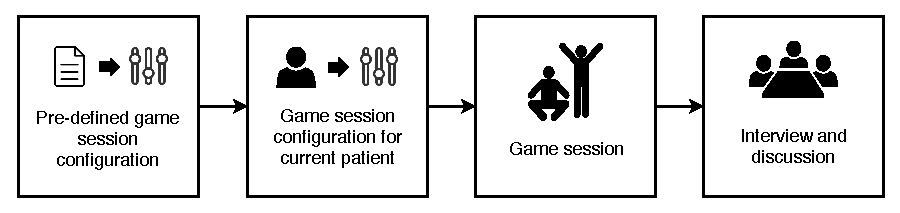
\includegraphics[width=.9\linewidth]{gfx/playtherapy/userOrientedEvaluation}} \quad
\caption{User-oriented evaluation to assess the interaction and effects moments of \ac{PX} in Playtherapy}
\label{fig:userOrientedEvaluation}
\end{figure}

\begin{figure}[bth]
\centering
\subfloat[\textit{B\'eisbol} evaluation session]{
   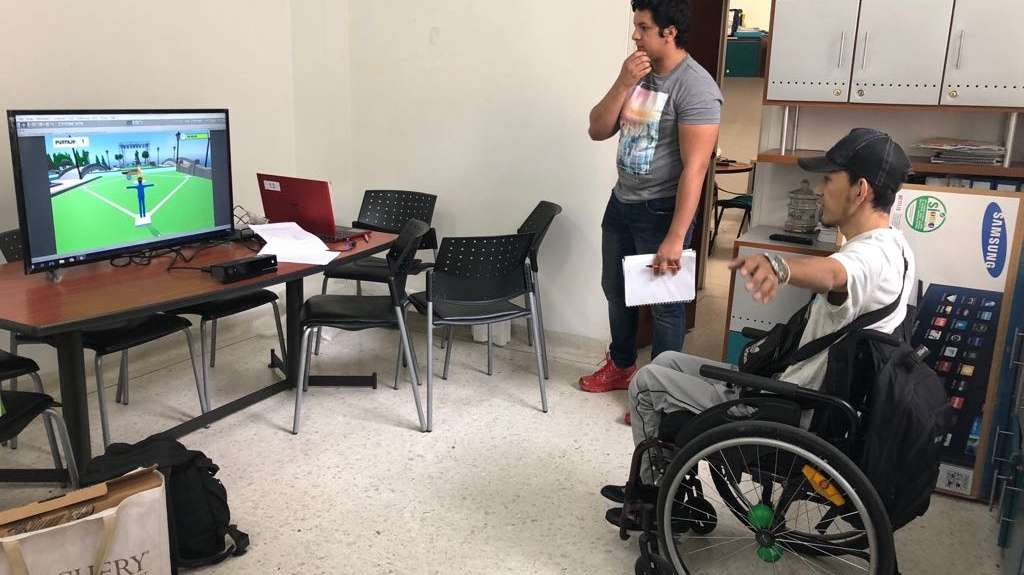
\includegraphics[width=0.4\linewidth, frame]{gfx/playtherapy/wheelchair_test}
   \label{fig:wheelchair_test}
}
\subfloat[\textit{Tiro Libre} evaluation session]{
   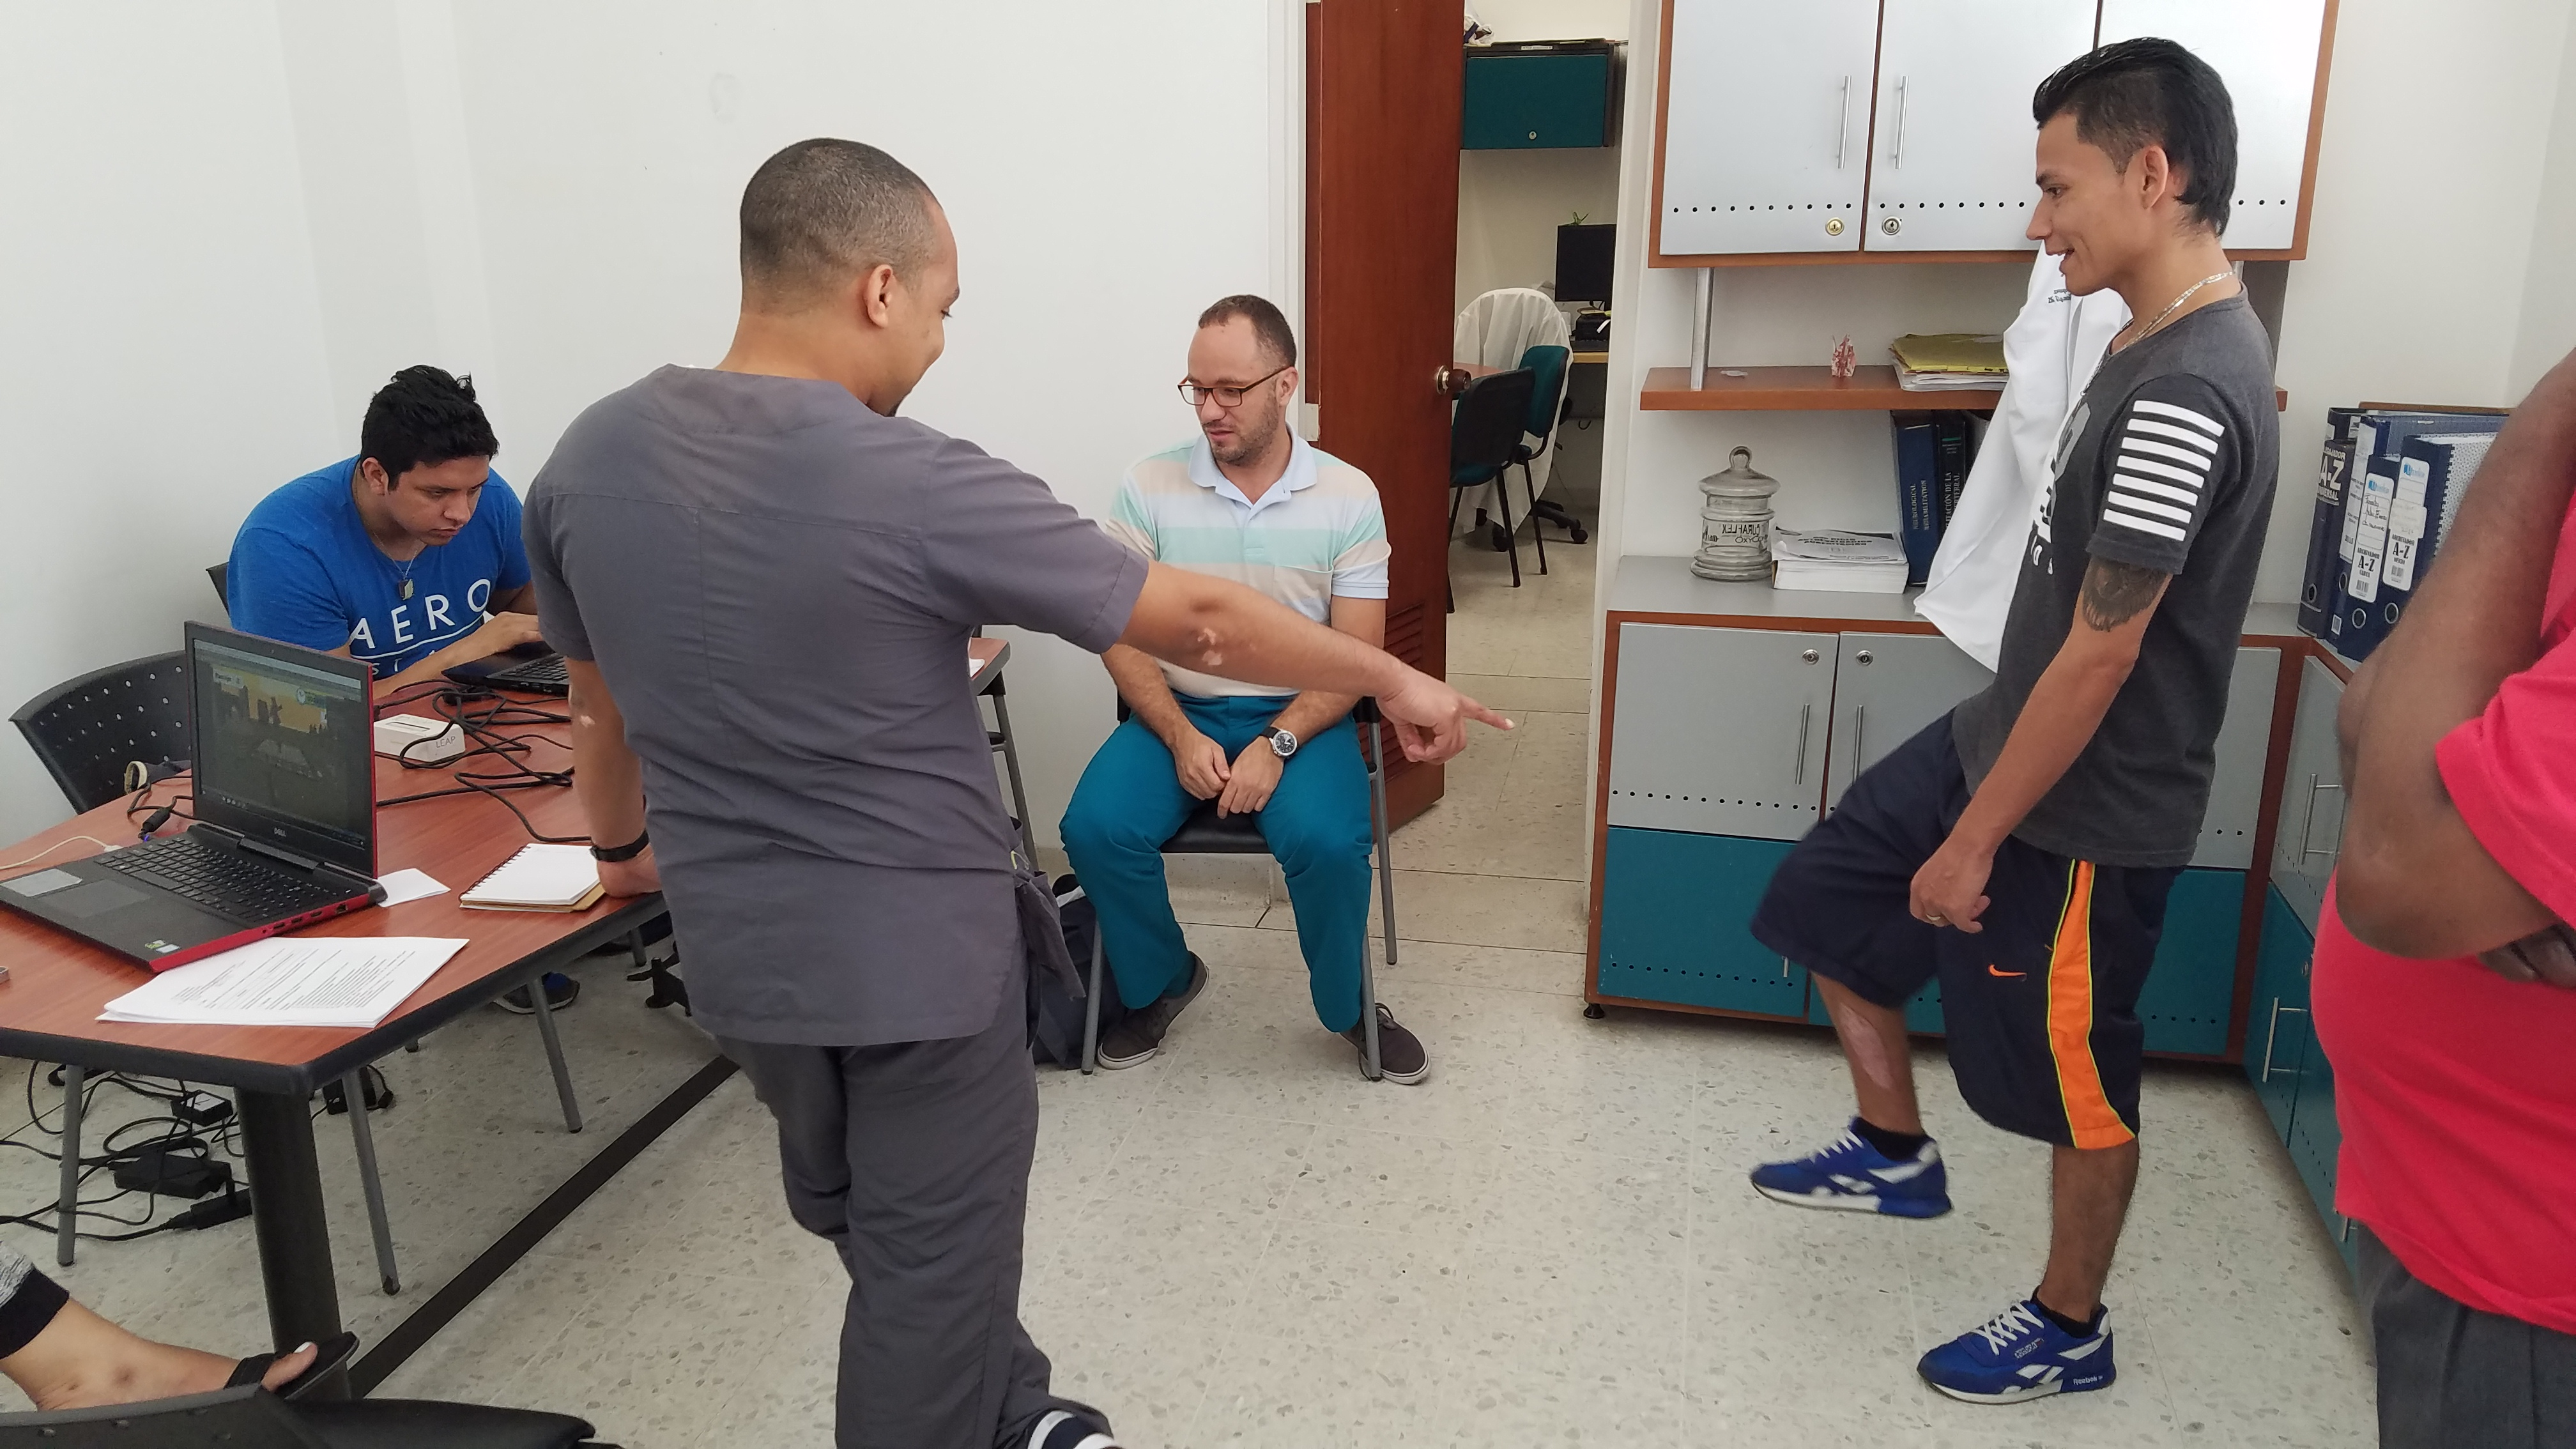
\includegraphics[width=0.4\linewidth, frame]{gfx/playtherapy/tiro_libre_test}
   \label{fig:tiro_libre_test}
}\\
\subfloat[\textit{Guerra Medieval} evaluation session]{
   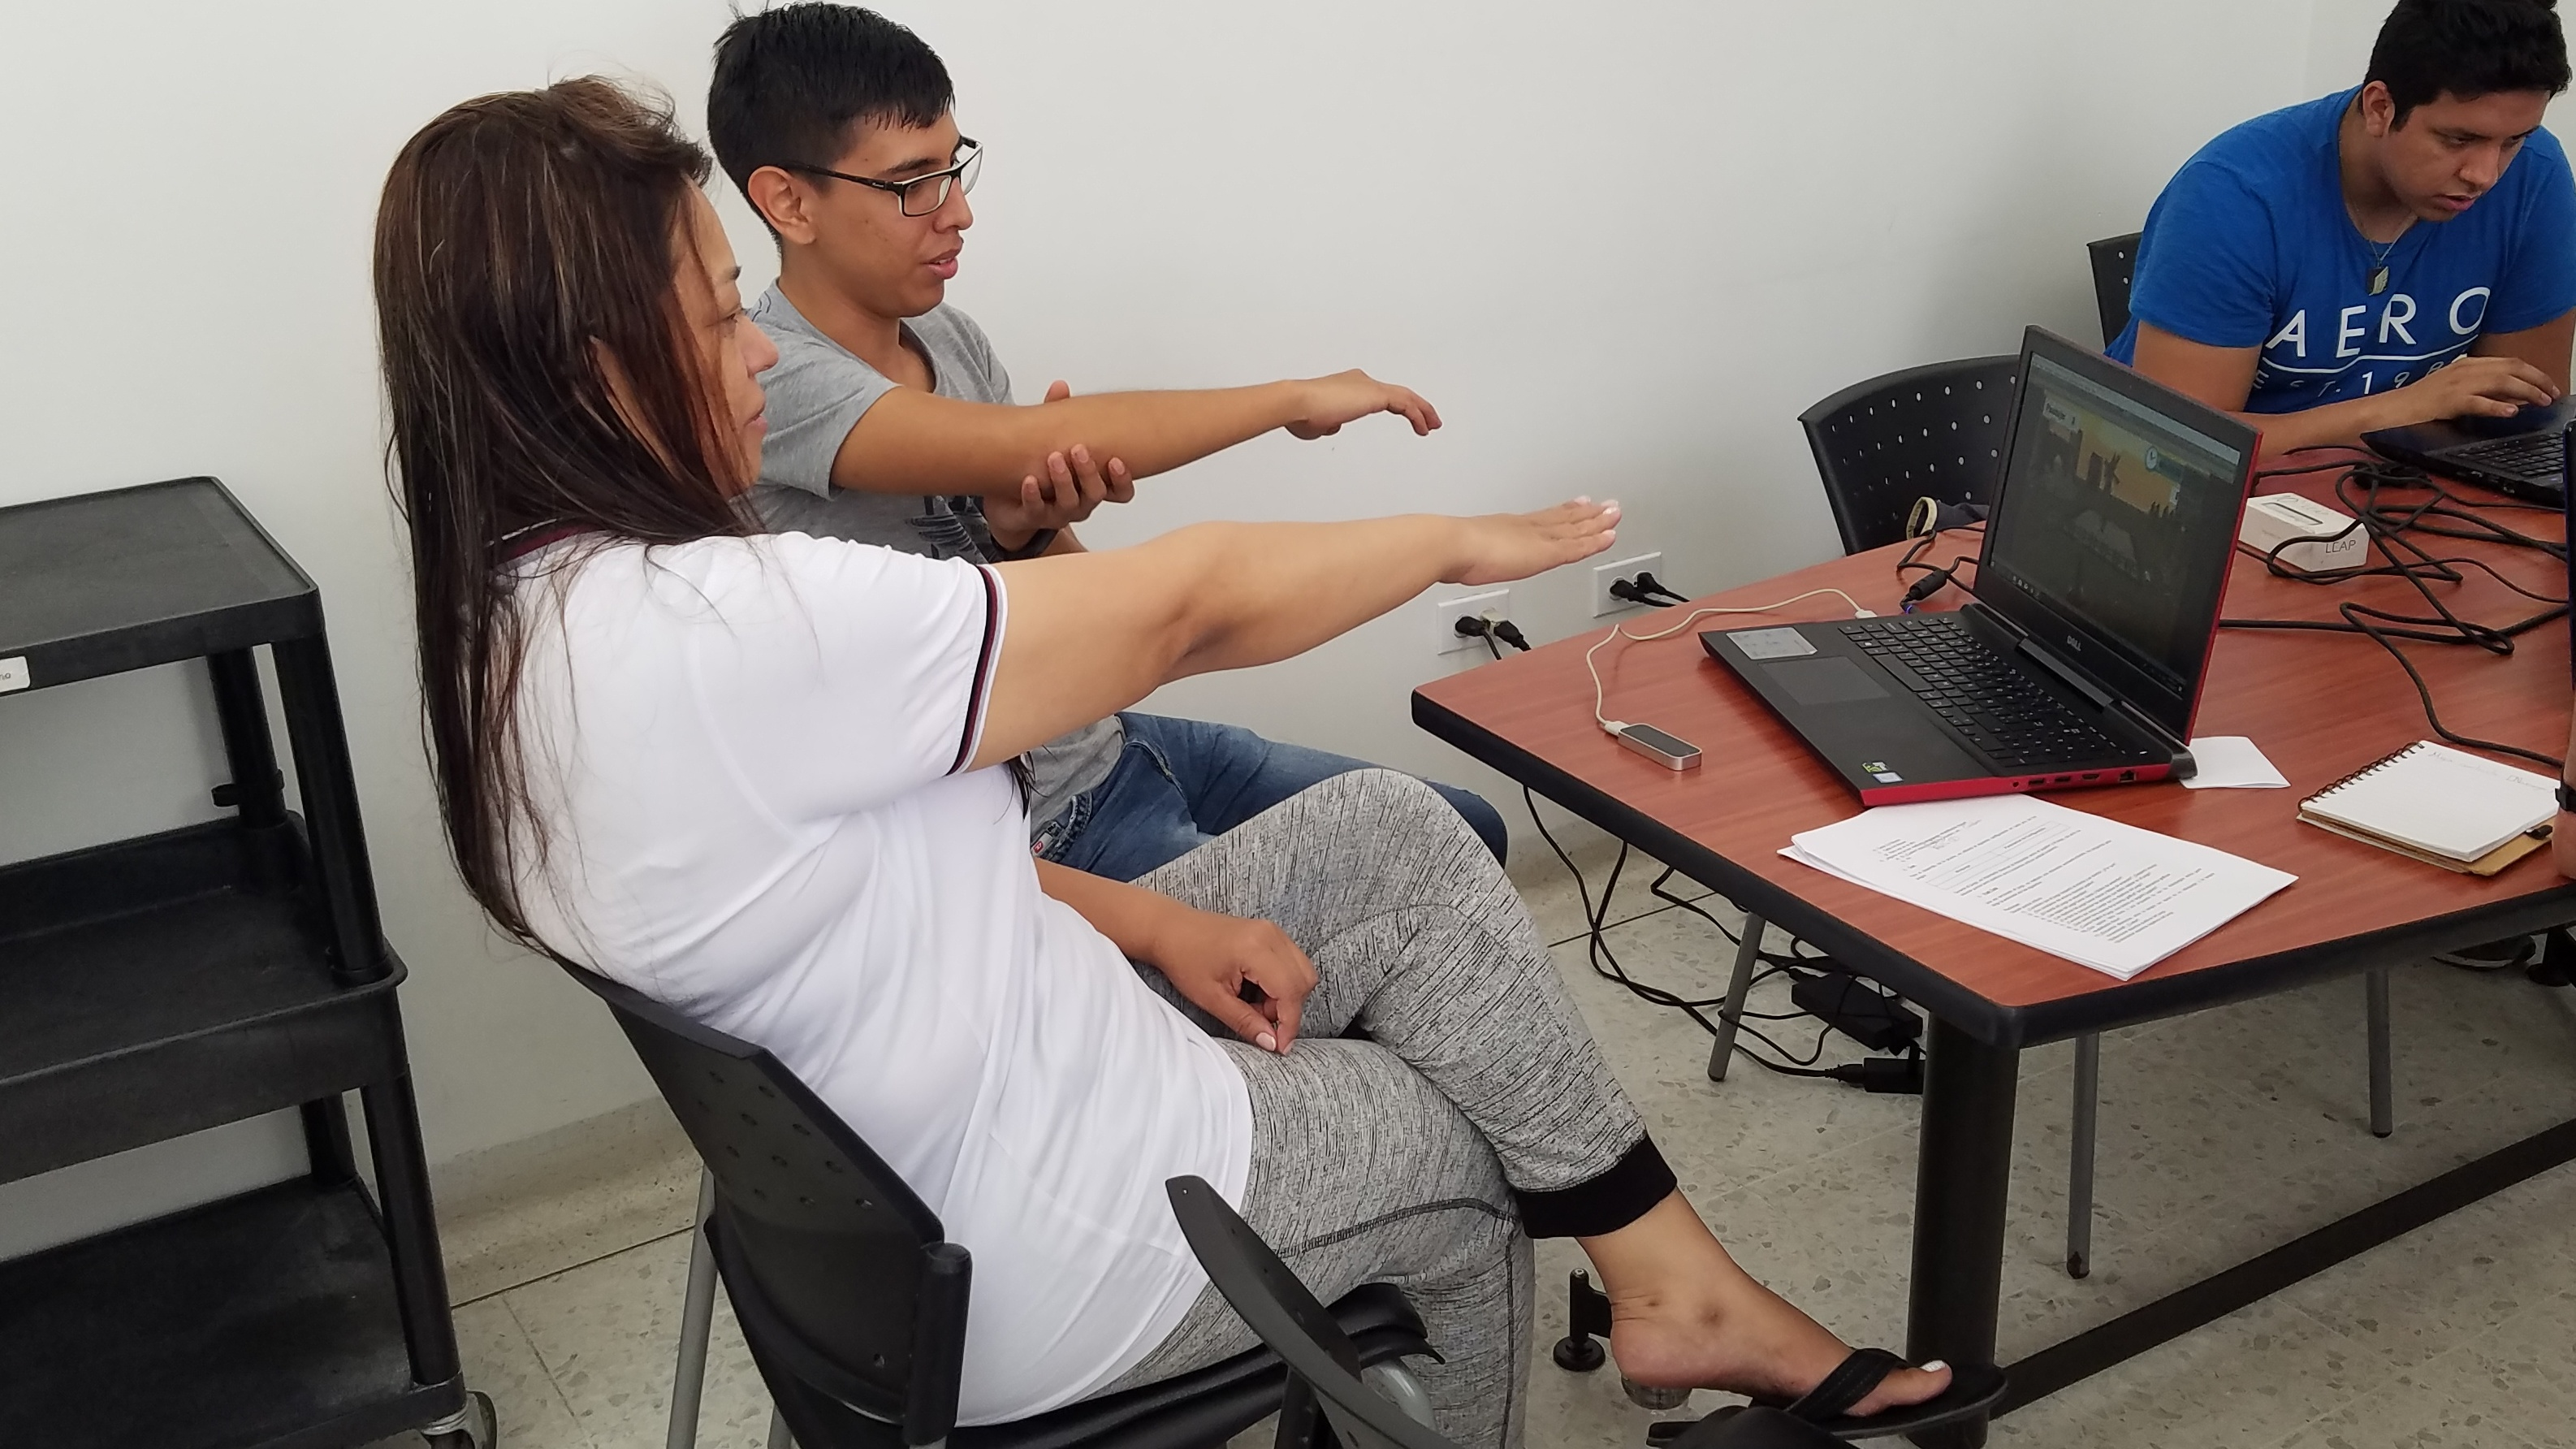
\includegraphics[width=0.4\linewidth, frame]{gfx/playtherapy/guerra_test}
   \label{fig:guerra_test}
}
\subfloat[\textit{Topos} evaluation session]{
   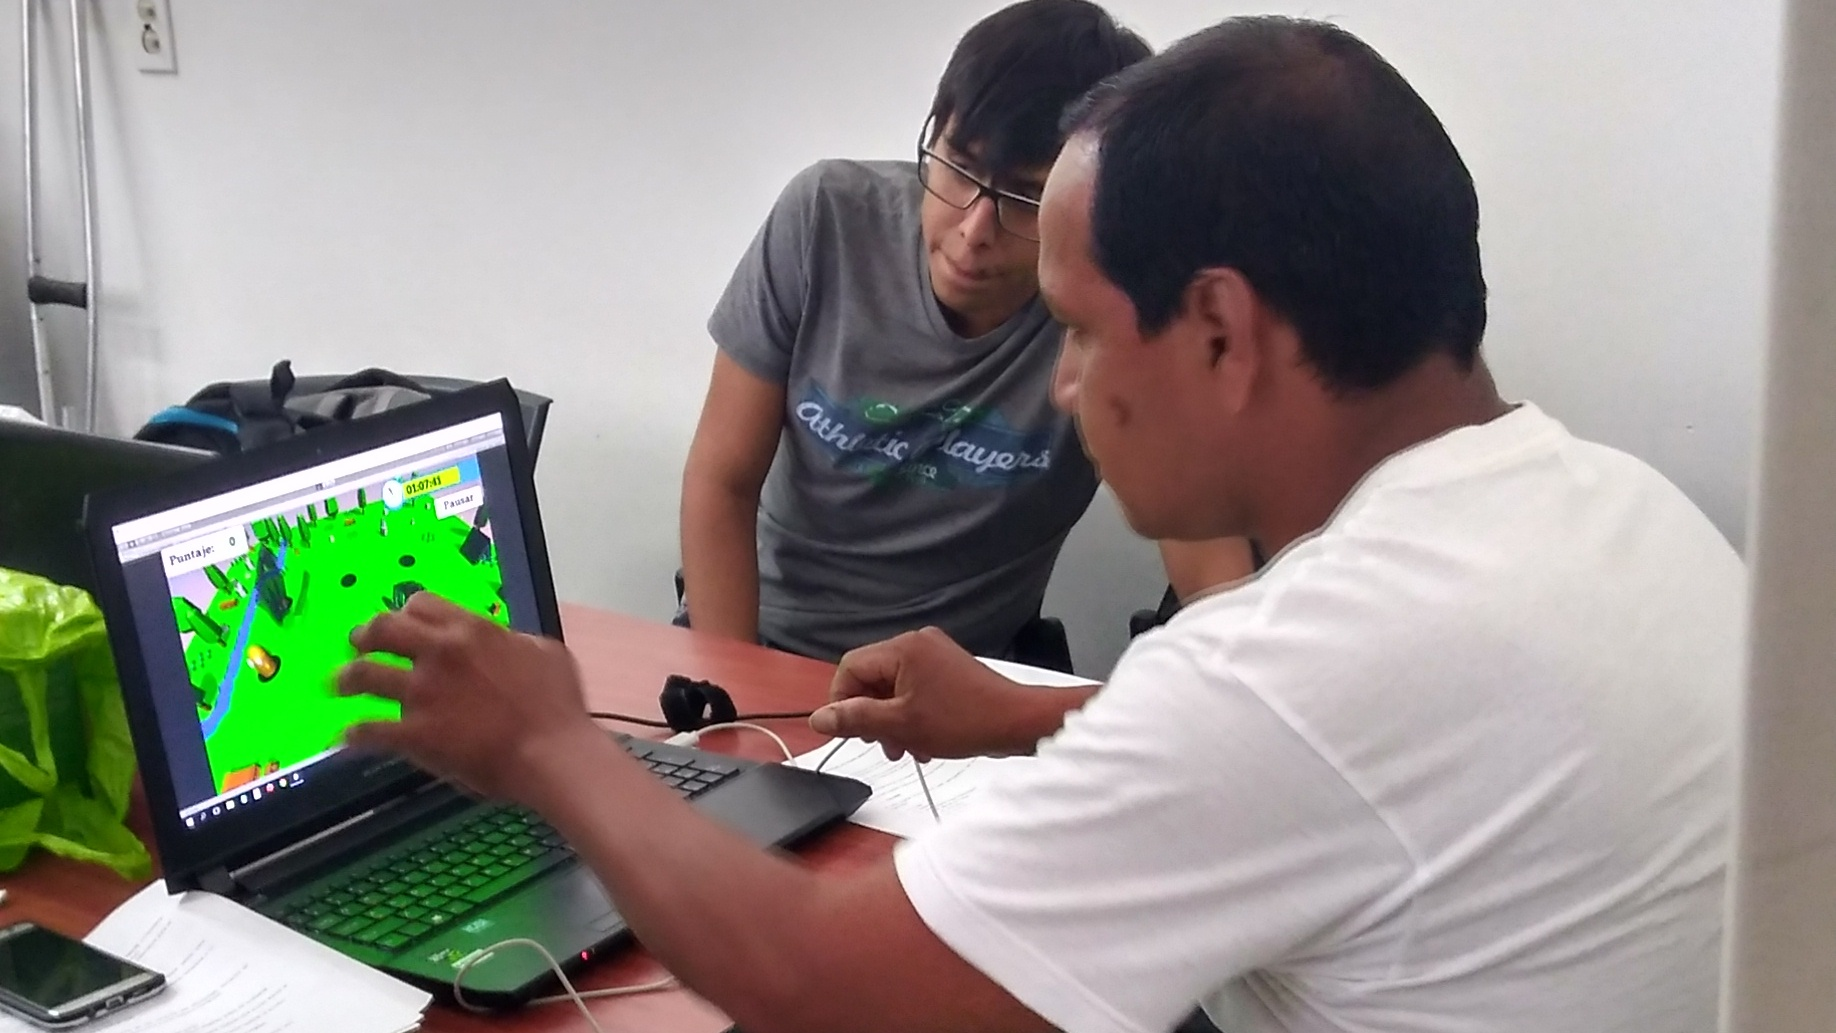
\includegraphics[width=0.4\linewidth, frame]{gfx/playtherapy/topos_test}
   \label{fig:topos_test}
 }
\caption{Evidence of some of the interaction and effects evaluation sessions}
\label{fig:evaluation_sessions}
\end{figure}

We interviewed the patients using the following questions:

\begin{enumerate}
    \item Did you enjoy playing the game?
    \item Were you interested in the game?
    \item Were you conscious about your environment while playing the game?
    \item Did you understand the game tutorial?
    \item Were the objectives, rules and movements of the game clear and easily understandable?
    \item What is your opinion about the graphical interface?
    \item What is your opinion on the use of digital games in physical rehabilitation therapy?
    \item What positive aspects did you find in the game?
    \item What negative aspects did you find in the game?
    \item Would you like to play again?
\end{enumerate}

Moreover, the questions that we employ for the interview with the physiotherapists are: 

\begin{enumerate}
    \item Was it easy for you to configure the game? Why?
    \item Did you like the overall appearance of the configuration screen? Why?
    \item What is your opinion on the use of digital games for physical rehabilitation therapy?
    \item What do you think could be the impact of Playtherapy in the field of physiotherapy?
    \item What positive aspects do you find in Playtherapy?
    \item What negative aspects do you find in Playtherapy?
\end{enumerate}

\subsubsection{Participants}
\label{sec:eval_int_eff_participants}

A total of sixteen people participated in the evaluation, nine men and seven women. They ranged in age from 19 years to 49 years ($M = 32.40, SD = 10.06$). One of the participants did not report his age. Verbal consent was obtained from them. A relation among the patients, the evaluated mini \acp{PREG} and the evaluation sessions is presented in \autoref{tab:participnats_interaction_eval}. Also, a reference to the report of each evaluation is included.

\begin{table}[bth]
\myfloatalign
\resizebox{.9\linewidth}{!}{
\begin{tabular}{lcl}
\toprule
\multirow{2}{*}{\spacedlowsmallcaps{Mini PREG}}
& \multicolumn{2}{c}{\spacedlowsmallcaps{Participants}} \\\cmidrule(r){2-3}
& \spacedlowsmallcaps{Physiotherapists} 
& \spacedlowsmallcaps{Patients (Age, Gender)} \\\midrule
Tiro Libre \autocite{Ruiz2017} & \multirow{2}{*}{1} & 1 (20, M) \\\cmidrule(r){3-3}
Rieles \autocite{Ruiz2017}  &  & 1 (40, F) \\\midrule
Piano \autocite{Ruiz2017}  & \multirow{2}{*}{1} & \multirow{2}{*}{1 (36, M)} \\
Topos \autocite{Ruiz2017}  &  &  \\\midrule
El Gran Viaje \autocite{DiMambro2017} & \multirow{3}{*}{1} & \multirow{3}{*}{3 (26, F; 23, F; 26, M)} \\
Vecinos Invasores \autocite{DiMambro2017} &  &  \\
Figuras Mágicas \autocite{DiMambro2017} &  &  \\\midrule
Cavano \autocite{Castillo2017} & \multirow{2}{*}{2} & \multirow{2}{*}{2 (19, F;  -, M; 27, M)} \\
Dulce Hogar \autocite{Castillo2017} &  & \\\midrule
F\'utbol Libre \autocite{Loaiza2017} & 1 & 3 (26, M; 40, F; 49, M) \\\midrule
B\'eisbol \autocite{Cortes2018} & \multirow{2}{*}{2} & \multirow{2}{*}{2 (47, F; 30, M)} \\
Defensa M\'agica \autocite{Cortes2018} &  &  \\\midrule
Guerra Medieval \autocite{Lopez2017b} & \multirow{2}{*}{2} & \multirow{2}{*}{2 (30, M; 47, F)} \\
Viajando en el Espacio \autocite{Lopez2017b} &  &  \\\midrule
\bottomrule
\end{tabular}}
\caption{Participants of the \ac{PX} evaluation sessions}
\label{tab:participnats_interaction_eval}
\end{table}

Additional demographic information was obtained for eight of the patients who participated in the evaluation, four men and four women. Their age ranged from 23 years to 49 years ($M = 33.38, SD = 10.39$). All patients needed to rehabilitate one or more body joints. Two patients were rehabilitating on of their knees, other two patients one of their shoulders, another one of his knees and feet, another one her hip, another one her spine, and the last one was treating muscular pain in her lower and upper limbs.

Four of the patients play digital games, one of them started playing less than 5 years ago, other two at least 6 years ago and the last patient more than ten years ago. Two of them play daily and the other two play weekly. Regarding their preferred platforms, one prefers arcade machines, other two PlayStation and the fourth one PlayStation, Xbox and arcade machines.

\subsection{Context}

\subsubsection{Environmental influences}
The evaluation sessions took place in a meeting room of the physical medicine and rehabilitation unit of the hospital since the \textit{location} where Playtherapy will be used was not defined yet.

We observed that physiotherapists became almost \textit{co-players} while the patients were playing. As expected, they monitored patients while they played. Additionally, they encouraged the patients and alerted them about game events (e.g. when an obstacle was approaching) in a very enthusiastic way (See \autoref{fig:tiro_libre_test}).

Only the 40 years old woman who played \textit{Rieles} said that she got distracted by the \textit{people around her}.

No \textit{assisting objects} were employed during any evaluation session.

\subsubsection{Rehabilitation environment}
The physiotherapists highlighted several characteristics of Playtherapy. The remarked that Playtherapy was flexible and practical since all mini \acp{PREG} can be configured to adapt to a patient needs. One physiotherapist said that it would serve as a creativity trigger because it allows working on additional aspects such as coordination, balance and self tempo-spatial location, which were not considered by the development team.

Furthermore, the physiotherapists describe Playtherapy as a suitable tool to bring variety and dynamism to the therapy sessions. Also, they claimed that the mini \acp{PREG} are easy o use. Thus, Playtherapy may be a source of motivation for patients.

They requested to fix the issues identified by the patients to offer a higher-quality experience. Moreover, they recommended including more mini \acp{PREG} to have even more alternatives and give patients the opportunity to play different mini \acp{PREG} with the same rehabilitation goals. Finally, the stated that including a screen to be able to register comments after each therapy session to provide patients with \textit{progress feedback}.

\subsection{Player/Patient}
Although the patients were shy and provided very basic answers even when we tried to go deeper in a question, we were able to collect general information about their cognitive and emotional processes and responses while playing a Playtherapy's mini \acp{PREG}.

\subsubsection{Cognitive and emotional processes}
\subsubsection*{Audiovisual appeal}
Patients evaluated the visual elements of Playtherapy's mini \acp{PREG} positively. They considered that the \ac{GUI} elements were clear and visible since the employed colours, fonts, controls (e.g. text fields, sliders, selectors and buttons) and panels were adequate (See \autoref{fig:platherapy_screens}). Also, patients claimed that the mini \acp{PREG}' low poly visual style was attractive.

Nonetheless, some suggestions for some mini \acp{PREG} resulted from the evaluations. Some patients suggested improving colour contrast in \textit{El Gran Viaje}, \textit{Figuras M\'agicas} and \textit{Rieles} due to visibility issues. For instance, two of the patients who played \textit{Figuras M\'agicas} were more concentrated on trying to identify the plane they should control rather than achieving the game goals.

\subsubsection*{Clarity of goals}
In general, the patients were able to understand the main goal of all mini \acp{PREG}. They claimed that the adopted themes were encouraging and clear.

Nevertheless, some games presented specific issues. The 49 years old man who played \textit{Figuras M\'agicas} stated that the visual aid that indicated which leg to move was not visible enough. Additionally, the 47 years old woman who played \textit{B\'eisbol} and \textit{Defensa M\'agica} had difficulties to understand and achieve game goals. Nevertheless, she could complete a successful game session after receiving instructions from a physiotherapist.

\subsubsection*{Immersion}
Most patients expressed that they concentrated on achieving the mini \acp{PREG} goals, forgetting the clinical environment and the fact that they were performing a therapeutic activity.

The man who played \textit{Piano} did it twice. In the first game session, the audio effects were accidentally disabled; once the physiotherapist realised about it, a second game session was started. As expected, the patient expressed that the audio effects improved the experience and got his attention.

\subsubsection{Cognitive and emotional responses}
In general, all patients agreed that including Playtherapy's mini \acp{PREG} in physical therapy may represent a motivating, enjoying and dynamic alternative to traditional activities. They claimed that these games might enrich their experience during their treatments.

Some of them highlighted the fact that these \acp{PREG} allow them to execute therapeutic exercises as a motivating aspect to use them. One patient remarked that she would not use games at home, though it would be an entertaining activity to be performed in therapy while working on her rehabilitation goals. The man who tested \textit{Topos and Piano} claimed that the most remarkable characteristic of both games was to be able to move his fingers. Those comments confirm that the sense of being able to progress is an important source of motivation for patients to use unconventional therapeutic activities.

\subsection{Game system}
\subsubsection{Rehabilitation support}
Playtherapy's mini \acp{PREG} are of second degree of autonomy (i.e., these are supervised). Consequently, \textit{monitoring and correction capability} are not expected to be evaluated since those tasks should be executed by a physiotherapist. The only requirement is that a mini \ac{PREG} should allow pausing the game session to correct patients or reconfigure parameters.
Therefore, we were interested in assessing the \textit{adaptation} capability through configuration. The parameter screen of twelve of the mini \acp{PREG} were evaluated using a predefined configuration (See \autoref{tab:configurations}). A physiotherapist received the expected configuration, then he/she had to configure a game session accordingly. As mentioned previously, their opinions were collected at the end of each evaluation session.

\begin{table}[tbh]
\myfloatalign
\resizebox{\linewidth}{!}{
\begin{tabular}{lp{16cm}}
\toprule
\spacedlowsmallcaps{Mini PREG}
& \spacedlowsmallcaps{Configuration} \\\midrule
Tiro Libre
& Set up the game for 30 repetitions, use only the frontal plane with the following activation angles: 30 for the minor, 50 for the intermediate and 70 for the high, use lateral shifts with 80\% frequency, time between targets by default and changing the movement in failure
\\\midrule
Rieles 
& Set up the game for a 2-minute session on easy difficulty, for the patient to have to raise the knees at least 10 cm and the time between rises to be 1.5 seconds maximum, for the patient to have to crouch at least 25 cm, jump at least 15 cm and with lateral shifts 
\\\midrule
Piano 
& Set up the game for 20 repetitions, without simultaneous hands, with a time between repetitions of 1 second and with the pinch game mode with a minimum path of 90\%
\\\midrule
Topos
& Set up the game for 1 minute and 30 seconds, with simultaneous hands, with a time between repetitions of 2 seconds, with a mole up-time of 2.5 seconds and with the touch game mode, including all fingers
\\\midrule
B\'eisbol
& Set up the game for 30 repetitions, with a 30\% of the maximum ball speed, let the player work with the left shoulder with a minimum angle of 30 and a maximum angle of 60 and do not allow elbow movements and lateral shifts
\\\midrule
Defensa M\'agica
& Set up the game for 2 minutes, let the player work on flexion of both shoulders, with a minimum angle of 30 and a maximum angle of 180
\\\midrule
El Gran Viaje
& Set up the game for 30 repetitions, with left and right trunk and lower limbs movements, with the following angles: 20 for the minimum frontal, 15 for the minimum lateral and 30 for the maximum lateral. Let the patient to rest for 8 seconds and do not request to keep the movement.
\\\midrule
Vecinos Invasores
& Set up the game for 30 repetitions, include 50 animals, let the player to rest for 3 seconds, use the simple touch mode involving all fingers.
\\\midrule
Figuras Mágicas
& Set up the game for 5 repetitions, let the player to rest for 5 seconds, request the player to use 50\% of the screen to draw and enable all figures. 
\\\midrule
F\'utbol Libre
& Set up the game for 2 minutes, let the player to work with the right foot, with a resting time of 8 seconds and angle range between 30 and 70.
\\\midrule
Cavano
& Set up the game for 3 minutes, with a ulnar deviation of 20 and a radial deviation of 10
\\\midrule
Dulce Hogar
& Set up the game for 3 minutes, with a ulnar deviation of 20 and a radial deviation of 10
\\\midrule
\bottomrule
\end{tabular}}
\caption{Configuration that physiotherapists set up to test the configuration capability of each mini \ac{PREG}}
\label{tab:configurations}
\end{table}

All the participant physiotherapists could configure the game sessions as requested and assessed the process as intuitive. They considered that most configuration parameters were clear and easy to understand. Also, they stated that the \ac{GUI} of the parameter screens had a nice appearance and the font format was adequate. They remarked that having the possibility to select and configure a list of mini \acp{PREG} to play in a game session was practical for planning and time management purposes.

Nevertheless, they had difficulty to understand some configuration parameters; accordingly, they recommended using visual aids (e.g., tool-tips) and composing a user guide to describe the purpose of each parameter.

\subsubsection{Functional characteristics}
\subsubsection*{Tutorial}
In general, patients an physiotherapists assessed all tutorials positively. They said that these allowed to understand the game mechanics, rules and therapeutic movements adequately.

\subsubsection*{Ease of Control}
For six of the games that use the Kinect as interaction device; i.e., \textit{B\'eisbol, Defensa M\'agica, El Gran Viaje, Figuras Mágicas, Rieles}; the patients agreed that controlling the mini \acp{PREG} was natural and easy since they should perform common daily-life (e.g. jogging and squats) or therapy (e.g. shoulder flexion and extension) movements. A particular case was the 30 years old man who played \textit{B\'eisbol} and \textit{Defensa M\'agica}, he was on a wheelchair and had no difficulty to play both mini \acp{PREG} achieving high performances.

Nevertheless, some of the patients who played \textit{Tiro Libre} and \textit{F\'utbol Libre} had difficulty to the achieve game goals and perform the required movements naturally. In both games, patients have to interact with a ball; however, the movements were not natural since the ball did not behave according to the force that patients applied to the ball.

Regarding \textit{Figuras M\'agicas}, although drawing the expected figure was easy for patients, they usually forgot to switch to the drawing mode by grasping their hands and finish it by clapping their hands. The patients suggested adding visual aids. 

Additionally, the 23 years old woman who played \textit{El Gran Viaje} could not play the hip mode, though the physiotherapist configured a new game session to adapt to the patients' skills. In the second session, she played the trunk mode of the mini \ac{PREG}.

Finally, the patients who tested the hands mini \acp{PREG} found it problematic to control the virtual hands at the beginning of each session. They needed some time before they could get used to the virtual world since they could perform movements in all three dimensions. In the case of the mini \acp{PREG} that use Kinect, this was not problematic because patients are not required to move freely in the virtual world.

\subsubsection*{Playability}

We employed the approach presented in \autocite{Sanchez2012} to evaluate the playability of Playtherapy's mini \acp{PREG} using a Heuristic evaluation method. For the purpose of our evaluation we \textit{selected a set heuristics} from \autocite{Desurvire2009,Federoff2002}. The selection was made considering the following two facts to exclude heuristics:

\begin{enumerate}
    \item Playtherapy's \acp{PREG} are mini-games since a therapy session takes one hour approximately, and other therapeutic activities should be carried out. Thus, complex stories, mechanics, worlds or levels are not desired.
    \item Playtherapy's \acp{PREG} are of second degree of autonomy. Accordingly, some game parameters such as time and difficulty are defined by physiotherapists to assure a safe achievement of rehabilitation goals.
\end{enumerate}

Two members of Playtherapy's development team and a usability engineering university teacher selected the final set of heuristics. One of the members was an undergraduate student whose final career project was on the usability and digital games field; also, he developed \textit{F\'ubol Libre} mini \ac{PREG}. The other member is the student who conducted this master project. The teacher has taught the usability engineering course at \textit{Universidad del Valle}, \textit{Tulu\'a} branch during three semesters. First, each of the evaluators selected a set of heuristics individually, indicating the reason to include or exude each heuristic in a spreadsheet file. Then, a meeting was arranged to discuss the individual selections and select the final set of heuristics to be employed for the evaluation, which is available online \footnote{Final heuristics selection: \url{https://goo.gl/9JU4Cr}}.

Then, all Playtherapy's mini \acp{PREG} were evaluated by three evaluators (See \autoref{tab:heuristic_evaluators}). The evaluated versions of the \acp{PREG} are the same as those tested by the patients. \textit{Evaluator 1} is the undergraduate student who participated in the heuristic selection. \textit{Evaluator 2} was the developer of \textit{Tiro Libre, Rieles, Piano} and \textit{Topos}. Finally, \textit{Evaluator 3} is the student who conducted this master project. The evaluators had to score each heuristic raging from $1$ (heuristic was not or poorly met) to $5$ (heuristic was completely met). The scores were registered in a spreadsheet template that calculates a global playability score, a score for each playability facet and a score for each playability attribute as suggested in \autocite{sec:playability}. The template was provided by one of its authors. The social playability facet was not evaluated since Playtherapy's mini \acp{PREG} are meant to be played individually. Furthermore, the personal facet heuristics were rated based on the feedback collected during the evaluation with the patients at the hospital. 

The final scores are interpreted as follows:

\begin{itemize}
    \item \emph{1.0 t0 2.9}: Critical, it means that the evaluated aspect represents a problem that should be fixed in the \ac{PREG}
    \item \emph{3.0 to 3.9}: Medium, it means that the evaluated aspect needs to be improved 
    \item \emph{4.0 to 4.4}: Acceptable, it means that the evaluated aspect is satisfactory but could be improved
    \item \emph{4.5 a 5.0}: Excellent, it means that the evaluated aspect is satisfactory
\end{itemize}

\begin{table}[bth]
\myfloatalign
\begin{tabular}{ll}
\toprule
\spacedlowsmallcaps{Mini PREG}
& \spacedlowsmallcaps{Evaluators} \\\midrule
Tiro Libre & \multirow{10}{*}{Evaluator 1} \\
Rieles & \\
Piano & \\
Topos & \\
El Gran Viaje & \\
Vecinos Invasores & \\
Figuras Mágicas & \\
Cavano & \\
Dulce Hogar & \\\midrule
F\'utbol Libre & Evaluator 2\\\midrule
B\'eisbol & \multirow{2}{*}{Evaluator 2 and Evaluator 3} \\
Defensa M\'agica  & \\\midrule
Guerra Medieval & \multirow{2}{*}{Evaluator 3} \\
Viajando en el Espacio & \\\midrule
\bottomrule
\end{tabular}
\caption{Participants of the \ac{PX} evaluation sessions}
\label{tab:heuristic_evaluators}
\end{table}

The results of the heuristic evaluation were positive in general. As observed in \autoref{fig:playability_score} all mini \acp{PREG} achieved a global \textit{playability} score over $4.0$. The scores raged from $4.07$ to $4.81$ ($M = 4.53, SD = 0.19$). Nine ($60.00\%$) of the \acp{PREG} achieved an \textit{excellent} score and the rest ($40.00\%$) reached an \textit{acceptable} score. The results of all mini \acp{PREG} and a summary are available online \footnote{Heuristic evaluation results: \url{https://goo.gl/axds7s}}.

\begin{figure}[bth]
\myfloatalign
{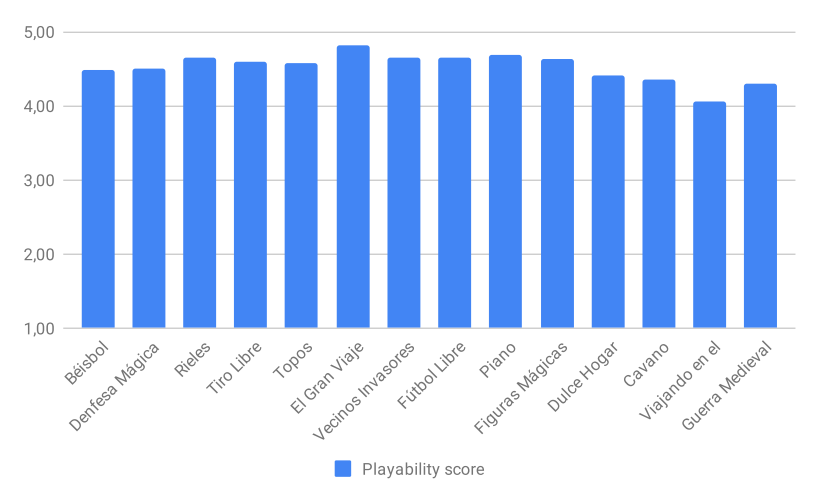
\includegraphics[width=\linewidth]{gfx/playtherapy/playability}} \quad
\caption{Playability score of Playtherapy's mini \acp{PREG} obtained from the heuristic evaluation}
\label{fig:playability_score}
\end{figure}

Regarding the \textit{playability facets} (See \autoref{fig:playability_facets}), the obtained scores raged from $3.52$ to $5.00$ ($M = 4.53, SD = 0.38$). Eleven mini \acp{PREG} ($78.57\%$) reached an \textit{excellent} score for the \textit{personal playability}, and the remaining three ($21.43\%$) achieved an \textit{acceptable} score. Similarly, ten mini \acp{PREG} ($71.43\%$) scored an \textit{Excellent} score for the \textit{artistic playability}, and the remaining four ($28.457\%$) achieved an \textit{acceptable} score. About the \textit{interactive playability}, eleven mini \acp{PREG} ($78.57\%$) reached an \textit{excellent}, two ($14.29\%$) scored as \textit{acceptable} and one ($7.14\%$) as \textit{medium}. The mini \ac{PREG} with the lowest interactive score ($3.52$) is \textit{Viajando en el Espacio}. The \textit{mechanic playability} was rated as follows, six mini \acp{PREG} ($42.86\%$) were rated as \textit{excellent}, six ($42.86\%$) as \textit{acceptable} and two ($14.29\%$) as \textit{medium}. The games with the lowest mechanic scores are \textit{Viajando en el Espacio} ($3.71$) and \textit{Cavano} ($3.74$). Finally, the \textit{intrinsic playability} was the lowest scored facet. Only three mini \acp{PREG} ($21.43\%$) were rated as \textit{excellent}, six as ($42.86\%$) \textit{acceptable} and five ($35.71\%$) as medium. Those games are \textit{Tiro Libre} ($3.99$), \textit{Viajando en el Espacio} ($3.95$), \textit{Guerra Medieval} ($3.89$), \textit{Topos} ($3.76$) and \textit{Piano} ($3.70$).

\begin{figure}[bth]
\myfloatalign
{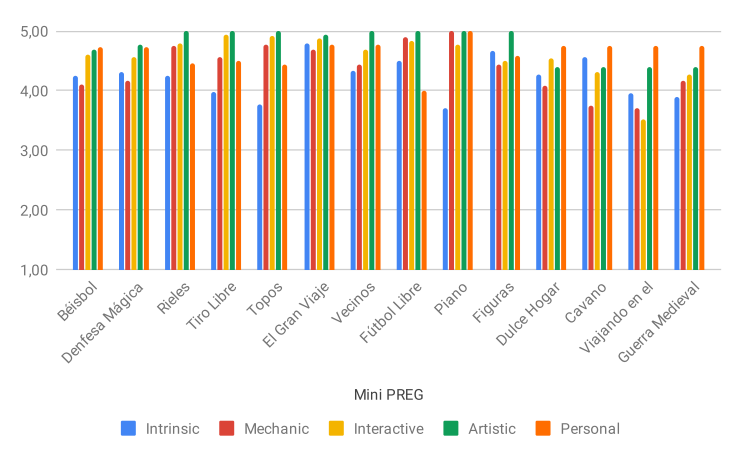
\includegraphics[width=\linewidth]{gfx/playtherapy/playability_facets}} \quad
\caption{Playability facets scores of Playtherapy's mini \acp{PREG} obtained from the heuristic evaluation}
\label{fig:playability_facets}
\end{figure}

About the \textit{playability attributes} (See \autoref{fig:playability_attributtes}), the scores minimum score was $3.04$ and the maximum was $4.95$ ($M = 4.50, SD = 0.33$). The mini \acp{PREG} were scored as follows. The best results were obtained for the \textit{immersion} attribute. Thirteen mini \acp{PREG} ($92.86\%$) were rated as \textit{excellent} and one ($7.14\%$) as \textit{acceptable}. Similarly, the \textit{emotion} attribute was scored as \textit{excellent} for twelve mini \acp{PREG} ($85.71\%$) and as \textit{acceptable} for the remaining two ($14.29\%$). \textit{Satisfaction} was rated as \textit{excellent} for eleven ($78.57\%$) mini \acp{PREG} and as \textit{acceptable} for the other three ($21.43\%$). The \textit{motivation} attribute was rated as \textit{excellent} for five mini \acp{PREG} ($35.71\%$), as \textit{acceptable} for seven ($50.00\%$), and as \textit{medium} for two mini \acp{PREG} ($14.29\%$), which are \textit{Dulce Hogar} ($3.97\%$) and \textit{Viajando en el Espacio} ($3.63\%$). Regarding \textit{learnability}, four mini \acp{PREG} ($28.57\%$) were rated as \textit{excellent}, nine ($64.29\%$) as \textit{acceptable} and one ($7.14\%$) as \textit{medium}. The lowest rated mini \ac{PREG} was \textit{Guerra Medieval} ($3.91$). Finally, two min \acp{PREG} ($14.29\%$) were rated as \textit{excellent}, nine ($64.29\%$) as \textit{acceptable} and one as \textit{medium}. The lowest score was for \textit{Viajando en el Espacio} ($3.04$).

\begin{figure}[bth]
\myfloatalign
{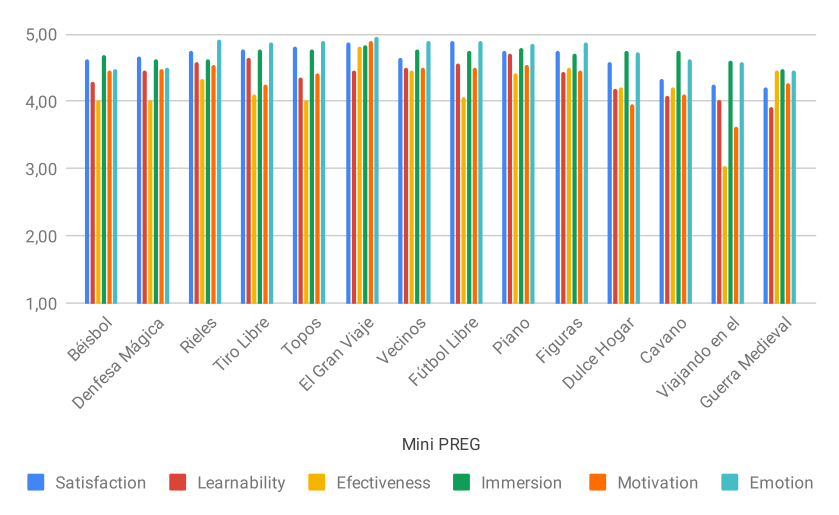
\includegraphics[width=\linewidth]{gfx/playtherapy/playability_attributtes}} \quad
\caption{Playability attributes scores of Playtherapy's mini \acp{PREG} obtained from the heuristic evaluation}
\label{fig:playability_attributtes}
\end{figure}

Although all the mini \acp{PREG} obtained a high global playability score, some aspects should be enhanced. Regarding the playability facets, the intrinsic one was the lowest rated. This facet is related to the gameplay design. Some of the selected heuristics require games to offer different mechanisms to interact and alternative or secondary goals. However, as stated previously, Playtherapy's mini \acp{PREG} have a quite simple design, in which complex interaction movements are not desired and gameplay time should be short (e.g., five to ten minutes) due to therapeutic reasons. The mini \acp{PREG} that provide more movement modes (e.g. \textit{El Gran Viaje} has two movement modes: trunk and lower limbs) rated the highest intrinsic score. The mechanical playability was the second lowest rated facet. In this context, some of the selected heuristics are related to players actions correction, game \ac{AI}, game elements interaction and save system. These aspects are desirable characteristics that are not implemented in Playtherapy's mini \acp{PREG} yet. Working on these aspects would improve Playtherapy playability.

\subsubsection{Progress data}

The results screen presents visual feedback after a game session depending on the players' performance (See \autoref{fig:results_screen}), it is based on the number of achieved goals (e.g. the number of caught balls in \textit{B\'eisbol}), which is closely related to the expected rehabilitation movements. Consequently, the physiotherapists and patients said that the screen is a simple way to have a sense of players' performance regarding \textit{game and rehabilitation goals}. Additionally, they said that presenting the best performance achieved by a patient might be encouraging.

Nonetheless, the physiotherapists recommended including an element to register observations after a game session. That may allow giving useful and personalised information about patients progress.

Playtherapy has an accompanying application which allows managing patients' information and visualising their progress throughout the game sessions. However, we did not test this application since it is not integrated into Playtherapy yet. Also, one interaction would not produce enough data to create meaningful reports.

\section{Discussion}

We presented how the proposed \ac{PX} model can be used to evaluate a \ac{PREG} (or a collection of \acp{PREG}). We evaluated Playtherapy using a multi-method approach that allow us assessing the three moments of \ac{PX} (i.e., \textit{antecedents}, \textit{interaction} and \textit{effects}) at the three levels of abstraction (i.e., \textit{context}, \textit{player/patient} and \textit{game system}) as suggested by the model we proposed in \autoref{ch:model}. The evaluation included different methods such as interviews, \ac{PREG} characterisation, Persona modelling, \ac{RITE} and Question asking protocol for the \textit{antecedents}. Furthermore, we employed question asking protocol, field observation, post-interview and heuristic evaluation for the \textit{interaction and effects} moments of \ac{PX}.

Compared to other evaluations, our work represents a comprehensive evaluation that comprises the whole \ac{PX} model. In general other evaluations have also employed a multi-method approach \autocite{Sinclair2010,Wuest2014,PirovanoAdvisor2012,Ni2014,Brokaw2015,Celinder2012,Hernandez2013,Shin2014,Moran2015,Chang2011,Rand2008,Fitzgerald2008,Saposnik2010}. Some of these works also conducted multi-stage or multi-study evaluations \autocite{Zhang2011,PirovanoAdvisor2012,Brokaw2015,Deutsch2011,Shin2014,Moran2015,Rand2008}. Regarding the layers of abstraction, the player and game system are commonly evaluated together \autocite{Wuest2014,Brokaw2015,Fitzgerald2008,Burke2009,Moran2015,Rand2008,Cameirao2010,Celinder2012}. Evaluating only the player layer may be a common practice \autocite{Sinclair2010,Zhang2011,Saposnik2010,Chang2011,Hernandez2013}. Some works have evaluated all three layers to some extent \autocite{Ni2014,Shin2014,Brokaw2015,PirovanoAdvisor2012}. Finally, although it is less common, game system evaluations are also reported \autocite{Deutsch2011, Sugarman2009}. Clearly, the less considered layer is context. About the moments of \ac{PX}, the three of them are commonly evaluated to some extent \autocite{PirovanoAdvisor2012,Wuest2014,Chang2011,Berkovsky2010,Hernandez2013,Celinder2012,Sugarman2009,Brokaw2015,Ni2014,Saposnik2010}. Two evaluations concentrated on the interaction and effect moments \autocite{Zhang2011,Rand2008}. Only one work focused on the antecedents moment of \ac{PX} to fully characterising a set of games for rehabilitation \autocite{Deutsch2011}. The antecedents mainly refer to the patients demographic and health characteristics and game system characterisations. Some of those evaluations also included previous experiences \autocite{Chang2011,Moran2015}. In general, the interaction layer assessed cognitive \autocite{Rand2008,Celinder2012,Hernandez2013,Shin2014,Fitzgerald2008}, emotional \autocite{Celinder2012,Sinclair2010,Zhang2011,Brokaw2015,Sugarman2009,Cameirao2010,Hernandez2013,Berkovsky2010,Moran2015,Rand2008,Burke2009}, and physical \autocite{Wuest2014,PirovanoAdvisor2012,Brokaw2015,Sugarman2009,Berkovsky2010} processes and responses for the player/patient layer, usability \autocite{Zhang2011,Celinder2012,PirovanoAdvisor2012,Brokaw2015,Cameirao2010,Moran2015,Fitzgerald2008} or rehabilitation support \autocite{Deutsch2011,Shin2014,Chang2011,Rand2008,Burke2009,Saposnik2010} for the game system layer, and cognitive processes \autocite{PirovanoAdvisor2012,Shin2014,Brokaw2015} (i.e. therapists thoughts and opinions) and inspired communication \autocite{Celinder2012} for the context layer. Which means that the proposed model may meet the requirements of \acp{PREG} evaluators and may contribute to be able to compare and assess evaluations comprehension and coverage in a consistent way.


% three moments: \cite{PirovanoAdvisor2012}, \cite{Wuest2014} (Interaction: ease of use, usefullnes, acceptance, adherence, attrition,, Effects (Physical, balance...)),Chang2011 (antecdenets, previous exp) Moran2015 also previous exp., Shin2014 physical responses, Berkovsky2010 8demographic questionnaire, physical reosnses, enjoyment), Hernandez2013 antecendentes (before trial, desinged, tested), interaction (emotional and physical processes),Celinder2012 Antecdents (health status)Interaction, Effects, Sugarman2009,Brokaw2015 (stroke impact). Ni2014: antecdents (level i an ii of gross motor function classification system GMFCS), no history of epilepsy, no injury that made physical act. unsafe, no viausl, cosgnitive or auditory disability, ability to comuunicat ein english or mandarin. Interaciont and effects (emotional)
% antec - inter, Sinclair2010,Fitzgerald2008,Burke2009,Cameirao2010 (IAntecedents (also validity of the system), interaction)



%- Inter -eff: Zhang2011,Rand2008: Interaction, Effects,
% antec,physical,Deutsch2011 

% player - game system: Wuest2014 (Interaction: ease of use, usefullnes, acceptance, adherence, attrition,, Effects (Physical, balance...)),Also antecedents, mainlyy health Brokaw2015 antecdents, player, system, context (pshysios, some opitnion s), stroke impact, pshysical effects,Fitzgerald2008,Burke2009,Moran2015,Rand2008, Cameirao2010 Player, game system (adaptation system was validated). IAntecedents (also validity of the system), interaction, Celinder2012 (Game system, Player/Patient (mainly) emotional acognitve processes,

% three layers: \cite{Ni2014}, Shin2014 (pshyiost and pisisathirs considered)(Contex, hopistal n o further dev, physios as informatns for design, player system),effects Celinder2012 (context, shrre expereinces with peers, familayi, firenda),Brokaw2015: player, system, context (pshysios, some opitnion s) , PirovanoAdvisor2012 Player, Game system, context (Clinicians)

% player: Sinclair2010, interaction, Zhang2011, Saposnik2010 (Interaction (exp, emotional), effects (physical),Chang2011,Hernandez2013)

% game system, Deutsch2011, Sugarman2009

%-------- antecedents
The antecedents evaluation allowed identifying a set of characteristics of the three layers of \ac{PX}, which served as a base for defining the scope of the following evaluations. After \acp{PREG} characterisation, the movements, parameters and modules to be assessed could be defined. Also, the players/patients and context characterisation determined which users should be involved in the user-oriented evaluation and which expectations and motivations should be evaluated. Furthermore, conducting \ac{RITE} testing sessions was an adequate strategy to identify issues as early as possible; that was confirmed by the second evaluation with a physiotherapist and a physiatrist who identified minor improvements in the mini \acp{PREG}. Accordingly, the results of the antecedents evaluation served as a guide for the Playtherapy's team throughout the whole development process to assure patients safety and a positive \ac{PX}. 

One limitation of the antecedents evaluation is the absence of patients participation to model Personas. We tried to overcome this limitation inquiring physiotherapists from the hospital about the patients' profile since they interact with them every day. Moreover, we complemented the initial Personas with the demographic information that we collected during the interaction evaluation in the hospital. Nonetheless, the low number of physiotherapists (three) who participated in the interviews, and the low number of patients (eight) who provided demographic data may be another limitation; though the collected data was coherent and consistent in both sources of information.

%-------- interaction
The results of the interaction evaluation were mainly positive. The most relevant reason for the positive results may be the use of a user-centred design process. Playtherapy was designed in collaboration with physiotherapists from the hospital in which it will be installed. They know the therapeutic needs, skills and expectations of the patients. Also, the developers followed a standardised development process that required them to implement a minimum set of components for each mini \ac{PREG}, leading to meet the identified needs and follow a similar structure (i.e., interaction means, art, \ac{GUI}, among others.). Furthermore, interaction devices such as the Kinect offer a natural way to interact as the patients expressed when they tested the mini \acp{PREG}.

Similarly, the antecedents evaluation serve as a reference to assure a high quality of \ac{PX}. Also, all mini \acp{PREG} have meaningful goals since these were designed to use the assisted rehabilitation movements as core mechanics; thus, patients achieve game goals while executing the expected rehabilitation movements. The mini \acp{PREG} provide rewards when patients complete each game goal, motivating patients to perform better. Moreover, every mini \ac{PREG} provides positive feedback when performing well, and encouraging feedback when not so well. 

Additionally, the physiotherapists remarked that one of the key features of Playtherapy is the parameters screen, available for each mini \ac{PREG}, which allows personalising a therapy session by setting configuration parameters according to the needs of a patient. The parameters screens were designed in collaboration with a physiotherapist from the hospital and the physiotherapy student who was part of the development team. Their participation resulted in a screen that meets physiotherapists expectations. Also, it makes Playtherapy a flexible tool that allows patients to concentrate on the joints and with the difficulty that they need. As described in \autoref{ch:characterising}, meeting physiotherapists expectations and patients motivation to progress in their recovery are key factors to encourage the use of a \ac{PREG} in physical therapy.

During the user-oriented interaction evaluation, we could confirm that older patients may have difficulties to understand new activities. The 47 patient who tested \textit{Defensa M\'agica} had to play twice since she could not understand the game rules. Before the second try, the accompanying physiotherapists explain her the game goals and the movements that she had to perform. That confirms the relevance of physiotherapists as guides and supervisors during game sessions conducted with Playtherapy. Nevertheless, that also indicates that some tutorials should include better animations and that the game should give clues when a patient is not having the expected performance.

% ------ effects 
Regarding the effects of \ac{PX}, we collected some data from patients and physiotherapists. The most relevant limitation is that the data derives from one game session. Consequently, most of them are short-term responses that may change after repeated use of a mini \ac{PREG}. Additionally, we did not assess physical responses since one episode may be not sufficient to obtain information about Playtherapy's impact on patients recovery process. That would require monitoring patients throughout a whole treatment. The only concluding result was that patients and physiotherapists were motivated to continue playing. They were enthusiastic at the fact that they could play a game while completing their rehabilitation treatments.

% ------ interaction and effects limitations
The interaction and effects evaluation has some limitations. First, although all people who tested the mini \acp{PREG} were patients from the hospital, in some cases they were not the target patients of a mini \ac{PREG} (e.g. one patient who tested \textit{Viajando en el Espacio} had a knee related impairment, but tested the trunk mode of this mini \ac{PREG}). Second, the evaluation sessions with patients and physiotherapists were not conducted in the room(s) where Playtherapy will be installed. Moreover, only \textit{B\'eisbol} and \textit{Defensa M\'agica} was tested with one of the TVs ($40''$) that will be used in the hospital, the other games were tested using laptops with $15''$ screens, which could difficult patients vision in mini \acp{PREG} the use Kinect. Lastly, the novelty of the employed technologies may be a reason for the positive feedback from patients since none of them had played using devices such as a Kinect or a Leap Motion.

Additionally, we conducted a heuristic evaluation to measure \ac{PX} quantitatively. The obtained results indicated that Playtherapy's mini \acp{PREG} could be enhanced regarding secondary goals, in-game help, story, \ac{AI} and additional interaction movements. However, those enhancements cannot compromise the level of control that physiotherapists have over the gameplay time and difficulty. Although the results of this evaluation were consistent with those obtained in the user-oriented evaluation, a limitation of this evaluation may be that most mini \acp{PREG} were evaluated by Playtherapy's developers, which could bias the results.
% Improvements
Additional improvements for Playtherapy includes (i) adding a monitoring system that assists patients when they are not having the expected performance or are executing movements incorrectly; (ii) adding an interactive tutorial or training levels for hands mini \acp{PREG} because patients need some time to get used to the 3D environment when interacting with a Leap Motion; (iii) the application to manage and visualise information associated to game sessions should be integrated with Playtherapy's mini \acp{PREG}, and (iv) exploring social possibilities to play Playtherapy.

The evaluations that we conducted allowed us to assess the antecedents and, to some degree, the interaction and effects moments of \ac{PX} offered by Playtherapy. However, to assess Playtherapy comprehensively, more patients should be exposed to the mini \acp{PREG} along a whole rehabilitation treatment. This would require monitoring the use of Playtherapy, e.g, conducting a clinical trial.

\section{Conclusion}
This chapter presented a \ac{PX} evaluation of a collection of \acp{PREG} called Playtherapy. We employed the methodology that we proposed in \autoref{ch:methodology} to perform the evaluation. As suggested by the methodology, we performed an iterative evaluation to be able to cover all layers and moments of \ac{PX} according to the model that we proposed in \autoref{ch:model}. Our initial goal was to assess the quality of Playtherapy to assure patients safety. Therefore, we focused on aspects such as configuration and movement mapping correctness while conducting an evaluation with one physiotherapy student, one physiotherapist and one physiatrist. Then we conducted a user-oriented evaluation and a heuristic evaluation, to assess the interaction and effects moments. We need to continue performing more evaluation iterations to test long-term effects and validate the results regarding interaction. The case study allowed us to confirm that evaluating the three layers of abstraction and the three moments of \ac{PX} in \acp{PREG} represents a big challenge since it takes time and effort before a single layer or moment can be covered. Also, it suggested that the proposed \ac{PX} model may meet the evaluation requirements of \acp{PREG}.